% !TEX TS-program = pdflatex
% !TEX encoding = UTF-8 Unicode

\documentclass[11pt]{report} % use larger type; default would be 10pt

\usepackage[utf8]{inputenc} % set input encoding (not needed with XeLaTeX)

%%% Examples of Article customizations
% These packages are optional, depending whether you want the features they provide.
% See the LaTeX Companion or other references for full information.

%%% PAGE DIMENSIONS
\usepackage{geometry} % to change the page dimensions
\geometry{a4paper} % or letterpaper (US) or a5paper or....
% \geometry{margin=2in} % for example, change the margins to 2 inches all round
% \geometry{landscape} % set up the page for landscape
%   read geometry.pdf for detailed page layout information

\usepackage{graphicx} % support the \includegraphics command and options

% \usepackage[parfill]{parskip} % Activate to begin paragraphs with an empty line rather than an indent

%%% PACKAGES
\usepackage{booktabs} % for much better looking tables
\usepackage{array} % for better arrays (eg matrices) in maths
\usepackage{paralist} % very flexible & customisable lists (eg. enumerate/itemize, etc.)
\usepackage{listings} % used here for code listing with syntax highlighting
\usepackage{color}

\definecolor{dkgreen}{rgb}{0,0.6,0}
\definecolor{gray}{rgb}{0.5,0.5,0.5}
\definecolor{mauve}{rgb}{0.58,0,0.82}

\lstset{frame=tb,
  language=Java,
  aboveskip=3mm,
  belowskip=3mm,
  showstringspaces=false,
  columns=flexible,
  basicstyle={\small\ttfamily},
  numbers=none,
  numberstyle=\tiny\color{gray},
  keywordstyle=\color{blue},
  commentstyle=\color{dkgreen},
  stringstyle=\color{mauve},
  breaklines=true,
  breakatwhitespace=true
  tabsize=3
}
\usepackage{verbatim} % adds environment for commenting out blocks of text & for better verbatim
\usepackage{subfig} % make it possible to include more than one captioned figure/table in a single float
\usepackage{float}
% These packages are all incorporated in the memoir class to one degree or another...
\usepackage{tikz-timing}
\usepackage{amsmath}
\usepackage{amssymb}

\usepackage{appendix}

%%% HEADERS & FOOTERS
\usepackage{fancyhdr} % This should be set AFTER setting up the page geometry
\pagestyle{fancy} % options: empty , plain , fancy
\renewcommand{\headrulewidth}{0pt} % customise the layout...
\lhead{}\chead{}\rhead{}
\lfoot{}\cfoot{\thepage}\rfoot{}

%%% SECTION TITLE APPEARANCE
\usepackage{sectsty}
\allsectionsfont{\sffamily\mdseries\upshape} % (See the fntguide.pdf for font help)
% (This matches ConTeXt defaults)

%%% ToC (table of contents) APPEARANCE
\usepackage[nottoc,notlof,notlot]{tocbibind} % Put the bibliography in the ToC
\usepackage[titles,subfigure]{tocloft} % Alter the style of the Table of Contents
\renewcommand{\cftsecfont}{\rmfamily\mdseries\upshape}
\renewcommand{\cftsecpagefont}{\rmfamily\mdseries\upshape} % No bold!

%%% END Article customizations

%%% The "real" document content comes below...

\title{LEAD -- Linux Embedded Automotive Dashboard}
\author{Esiri Igbako, Amal Kakaiya, Simon Jouet}
%\date{} % Activate to display a given date or no date (if empty),
         % otherwise the current date is printed 


\begin{document}
\maketitle
\newpage
\tableofcontents
\newpage

\chapter{Introduction}
	Formula Student (FS) challenges university students from around the world
	to design and build a single-seat racing car, which is then put to the test
	at the world famous Silverstone Circuit. \\
	\\
	At the University of Glasgow, the UGRacing team is the University's effort
	to provide a competitive car.
	The racing car is a collaborative effort by both the Mechanical 
	Engineering and 
	Electronic and Electrical Engineering departments. The fourth year team
	projects in Electrical and Electronic Engineering try to provide 
	electronic subsystems for the vehicle. This team, Team LEAD (Linux 
	Embedded Automotive
	Dashboard) were tasked with designing and building a display for the 
	dashboard
	using a provided USB Display. This report details the 
	research, design and implementation cycles involved in the creation of the
	final product.
	
	\section{Acknowledgements}
	The team would like to acknowledge, (in no particular order) the contributions
	 made by the following
	people. Their help has been greatly appreciated.
	\begin{itemize}
		\item Dr Muir
		\item Prof Ironside
		\item Nick Scott
		\item Liam MacIssac
		\item Iain Young
		\item Jordan Mellon
		\item Charlene Wilson
		\item Dingkun Ren
		\item The Gumstix users group
		\item Scott Ellis
		\item Linus Torvalds (for Linux)
		\item Richard Stallman (for the GNU GPL)
	 \end{itemize} 
	
			
	\section{Specifications}
	Following a discussion with UGRacing team members a formal technical
	specification of the final product has been defined as follows.
	
	\begin{itemize}
		\item The display must operate with the car's on board CAN bus to
		retrieve data to display.
		\item The following information must be displayed on the screen, speed
		revolutions per minute (rpm), fuel level, gear position and warning
		indicators from data provided by the vehicle CAN bus.
		\item The display should be configurable through hardware buttons to 
		allow a user to change some configuration settings such as units of
		measurement (e.g. mph to kph).
		\item The display should be easy to read using a high contrast colour
		scheme, to be legible and clear from the driving position.
		\item The system should include a diagnostic menu to provide 
		information about all the received CAN packets even the ones not 
		displayed on the main screen.
		\item The system should include if possible a CAN Bus packet data 
		logger as a side project.
		\item The CAN Bus interface should be compliant with ISO 11898
		(CAN Standard).
		\item Warning lights for coolant and oil temperature which flash when
		warning level (configured in the configuration menu) is reached.
		\item Flashing fuel indicator when less than a configured warning level
		is reached.
		\item Gear shift charge state indicating the electronic gear shift
		system charge level.
	\end{itemize}
	
	\section{Constraints}
	The UGRacing team also set some limitations on some factors of the system,
	primarily:
	
	\begin{itemize}
		\item Limit the power consumption as low as possible, below 1.5A
		including the power provided to the screen.
		\item Scale the device to the smallest package as possible to be able
		to fit it in the dashboard allocated space.
		\item The final system should be weather and vibration proof. It also
		should be robust to misuse (i.e. prevent mis connection).
	\end{itemize}

\chapter{Hardware System Design}
	\section{Introduction}
	The hardware for the dashboard had to address several criteria to be 
	able to
	retrieve, process and display the information provided by the car sensors. 
	The
	main requirements specify that the screen (see \ref{sec:screen} for more
	information) must use a USB port and allow to display an 800x480 image with
	a 16 bit depth colour. Another critical requirement was to implement a CAN
	interface as the dashboard should connect to the car CAN bus to retrieve 
	data.\\
	\\
	From these initial critical requirements, the team identified potential
	components of the hardware such as a CAN 2.0b compliant interface to 
	interface
	with the car sensors and an USB High Speed interface to connect the screen.
	Another criteria while designing the hardware was to create a flexible 
	system
	that can be extended or reallocated if required without any significant
	modifications of the circuit.\\
	\\
	In the following sections the different components of the hardware will be
	described with their description and purpose in the design.

	\section{Overview}
	An overview of the hardware architecture can be seen in \ref{fig:hardware_diagram}
	and represent the different stages and components used to develop the expansion
	board. The LCD displayLink Interface is provided through a USB connector and the
	serial debug port is available on a breakout board. The arrows and their directionalities
	represent the different communication/connection between the modules and
	describe if the communication is one or two ways.
	\begin{figure}[H]
		\centering
		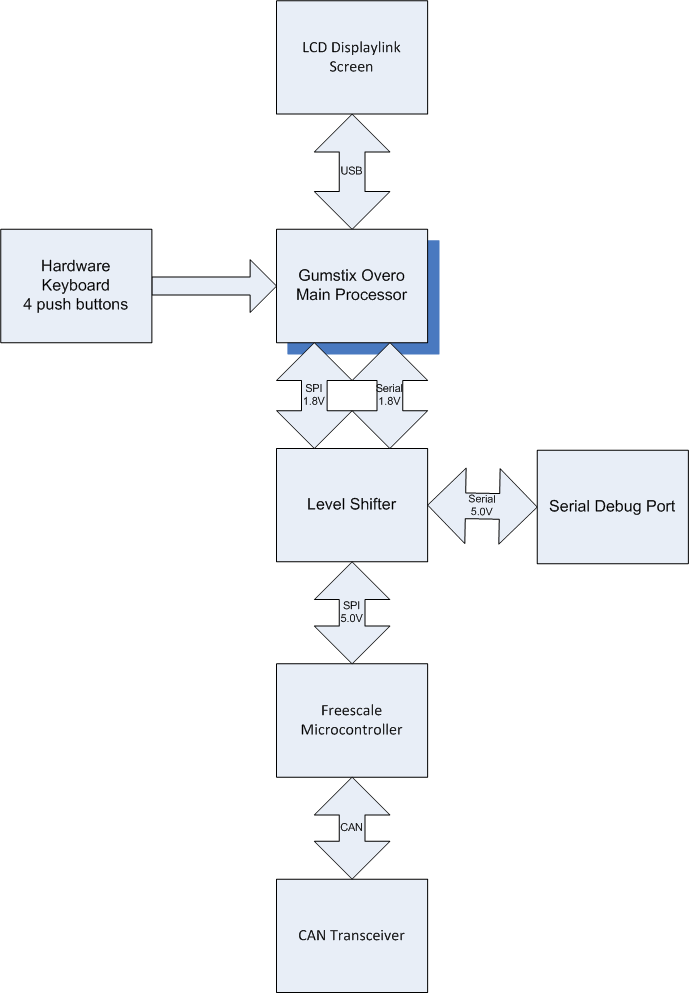
\includegraphics[scale=0.45]{images/hardware_diagram.png}
		\caption{Hardware Overview}\label{fig:hardware_diagram}
	\end{figure}
	
	\section{Gumstix}
		\subsection{Description}
		The main controller of the circuit is a Gumstix Overo Earth Computer on
		Module (COM) that provides a high processing power for a relatively
		low price. This module has been selected for the following 
		characteristics.
	
		\begin{itemize}
			\item Designed to run a GNU/Linux Operating system with an open source
			development toolkit.
			\item USB Host and On-The-Go ports provided
			\item Support of SPI and large number of General Purpose Input/Output 
			pins
			\item High clock speed of 600MHz and up to 1200 Million instructions
			executed per second (MIPS).
			\item On board RAM and NAND of 256MB.
			\item A low power consumption (less than 350mA) on high CPU load.
			\item Open design of the existing commercial expansion board to 
			facilitate the design of custom expansion boards.
			\item On board micro SD card to use as file system
			\item Small size board of 1.7 by 5.8 centimeters.
			\item Large open development community that could help to support
					development.
			\item Dock connectors can be used to build custom expansion boards
				to provide I/O to the gumstix.
			\item The Gumstix has been tested to meet the US Military standards
				MIL-STD-810 for vibration.
		\end{itemize}
	
		The Gumstix though, does not provide all of the features to match the initial
		specification. Such as the following:
	
		\begin{itemize}
			\item Does not have a built-in CAN Bus support
			\item Requires different voltages to operate, 3.3V for the 
			processor and 1.8V source for logic on the I/O pins.
			\item In addition, a 5V source is required for the USB connector.
		\end{itemize}
	
		However, due to the availability of the dock connectors and an open
		community of Gumstix users. We could build our own custom expansion
		board to provide the missing functionality.
	
		\subsection{Alternative Solutions}
		The team looked for other possible modules to use the USB screen.
	
		\begin{itemize}
			\item The Arduino Mega board is another low cost COM chip, however this 
			was quickly ruled out as the
			processing power is limited to 16MHz with 20 MIPS, and the on board ram
			of 8kB is not enough to store a single frame for the screen; assuming
			a raw picture at least 800 x 480 x 16 / 8 = 768kB of ram is required
			for a 800 by 480 with a 16 bit depth image.
		
			\item The BeagleBoard which runs on an OMAP 3530 processor, which is 
			basically the same
			processor as the one on the gumstix but with extra features such as
			hardware acceleration of openGL. The reason it has not been used is
			that the surface of the board is fairly large, 8 by 8 centimetres in the
			latest version.
		
			\item The last possibility was the Variscite COM that is similar to
			the gumstix but adds useful input/outputs protocols such as CAN. 
			However this product has not been used because the documentation is
			really limited and the expansion boards are not open to the community
			therefore increasing the chances of incorrect hardware. 
		\end{itemize} 
	
		\subsection{Purpose}
		The Gumstix is the main component of the hardware as it provides the USB
		interface to the screen and by being able to run a full distribution of
		GNU/Linux simplifies the programming by abstracting the access to the
		hardware and provide already developed drivers such as DisplayLink.\\
		In addition, it provides a solid testing platform for future development
		should extra software functionality be required. This is because new 
		software
		can be easily implemented, integrated, tested and 
		debugged on the gumstix.
	
	\section{USB Screen}
	\label{sec:screen}
		\subsection{Description}
		The Screen provided for the project is Lilliput UM-70C with a standard
		DisplayLink interface used for the communication, therefore any screen with
		this protocol should work directly on the dashboard without any hardware
		or software modifications. The screen's specifications are as following.
	
		\begin{itemize}
			\item USB only power source
			\item Screen resolution of 800 x 480
			\item Screen dimensions of 188 x 123 x 25.8 mm
		\end{itemize}
	
		However this screen has some limitations for the project
	
		\begin{itemize}
			\item High power consumption, requires almost 1A to operate and
			therefore the power consumption can reach 4.5W.
			\item This version of the screen does not have a touchscreen interface
			therefore limiting the interaction with the software to the hardware
			buttons.
			\item Too large to fit on the dedicated dashboard space on the car.
			\item Requires two USB ports to be able to provide 1A, 500mA per port. 
					[It can be noted though, that in testing it could operate off 
					one USB port alone.]
		\end{itemize}

	\subsection{Processing Requirements}
	The screen requires some memory to store the picture buffer on the  
	controller
	side and also CPU cycles to draw them into the frame buffer. These  
	calculations
	are based on the assumptions that the memory for the frame buffer is packed  
	(contiguous memory allocation) and
	that there is no padding spaces (no unused memory segment in the allocated 
	buffer) it is also assumed that 1 clock cycle is required to draw one pixel in
	the framebuffer, this delay is probably optimistic in most cases but due to 
	the presence of cache and DMA channels the exact timing can vary.\\
	\\
	\begin{center}
	Therefore the memory usage for the screen provided is:
	\begin{equation}
	\aligned
	Memory &= Width \times Height \times Bit Depth\\
	&= 800 \times 480 \times \frac{16}{8}\\
	&= 768,000 = 768kB
	\endaligned
	\end{equation}

		And the number of clock cycles required is:
		\begin{equation}
		\aligned
		Instructions &= 800 \times 480\\
		&= 384,000
		\endaligned
		\end{equation}

		To get a smooth display of the screen the framebuffer should be updated at
		least 25 times a seconds:
		MIPS (Million of Instruction Per Second) required
		\begin{equation}
		\aligned
		MIPS &= \frac{frame rate \times instructions per frame}{1,000,000}\\
		&= \frac{25 \times 384,000}{1,000,000}\\
		&= 9.6
		\endaligned
		\end{equation}

		CPU usage of the display on the gumstix processing power
		\begin{equation}
		\aligned
		Usage &= \frac{9.6 \times 100}{1200}\\
		&= 0.8 \%
		\endaligned
		\end{equation}
		\end{center}
	
		From these calculations we can estimate that the Gumstix system will not
		only have
		enough processing power to refresh the screen at the desired rate, but has
		plenty more power in reserve for background processes and tasks.
	
	\section{CAN Interface}
		\subsection{Description}
		The CAN interface as described earlier was a critical part of the design as
		the dashboard information depends on it, therefore an large amount of time
		as been dedicated to research different methods of accessing the CAN 
		network.\\
		\\
		The final software support two methods for accessing the CAN network, the 
		first
		one is through a CAN-USB adapter by Lawicell and the second one through an
		onboard Freescale microcontroller. The second method is the preferred one  
		as
		no external device to the expansion board is required and the onboard
		microcontroller can be reprogrammed to extend the functionalities of the
		dashboard, also the overall cost of the microcontroller is less than the 
		CAN-USB adapter.\\
		\\
		The microcontroller is interfaced to the gumstix through SPI with the  
		Gumstix
		as the master and the microcontroller as the slave. For the devices to 
		communicate a custom protocol has been designed in a request/reply type
		where one side requests
		information and the other one sends them if possible, also a burst mode has
		been implemented where a stream start command packet is sent by one side  
		and
		the other side sends as much information as possible from its internal 
		buffer.
		The burst mode has been implemented to remove the overhead of the 
		request/reply method. The SPI protocol specification can be seen in more
		detail in section \ref{sec:spi_proto}.	\\
		\\
		Using a microcontroller as the controller for the CAN bus provides a large
		buffer space to queue the packets before they can be retrieved by the 
		Gumstix.
		By using this technique the number of interruption to do Input/Output 
		operation
		is kept low and therefore the CPU throughput is higher. The microcontroller
		selected is the Freescale MC9S08DZ60 which has 4096 bytes of available RAM.
		We can therefore calculate the maximum queue size assuming all memory can be used for 
		queuing,
		and the CAN packets have an 11 bits identifier with up to 8 bytes of data.

		\begin{equation}
		Packet Size = Identifier(11) + DLC(4) + Data(64) + Overhead (2) = 81bits
		\end{equation}

		For performance improvement align each packet on a 8 bit memory space
		\begin{equation}
		Packet Size = 11 bytes
		\end{equation}

		Therefore maximum number of packets that can be queued
		\begin{equation}
		Q = \frac{RAM}{PacketSize} = \frac{4096}{11} \approx 372
		\end{equation}

		On the Formula Student car the data rate is set to 125Kb per second, therefore the
		maximum used data rate is

		These calculations are approximate as the transmission can be larger due to CAN
		Interframe spacing that can be at least three consecutive bits and also due to
		the bit stuffing extra bits can also be added.

		Assuming minimum CAN packet size (no data, more overhead)
		\begin{equation}
		\begin{aligned}
		PacketSize &= \sum{Frame\_Fields}\\
		&= 1 + 11 + 1 + 1 + 1 + 4 + 0 + 15 + 1 + 1 + 1 + 7 \\
		&= 44bits
		\end{aligned}
		\end{equation}

		\begin{equation}
		\begin{aligned}
		UsedData &= ID + DLC\\
		&= 11 + 4\\
		&= 15bits
		\end{aligned}
		\end{equation}

		\begin{equation}
		\begin{aligned}
		Overhead &= PacketSize - UsedData\\
		&= 44 - 15\\
		&= 29bits\\
		&= 66\%
		\end{aligned}
		\end{equation}

		\begin{equation}
		\begin{aligned}
		PacketsPerSecond &\approx \frac{bit rate}{PacketSize}\\
		&\approx \frac{125,000}{44}\\
		&\approx 2841
		\end{aligned}
		\end{equation}

		\begin{equation}
		\begin{aligned}
		SPIRequiredSpeed &\approx PacketsPerSecond \times UsedData\\
		&\approx 2841 \times 15\\
		&\approx 42615\\
		&\approx 43kHz
		\end{aligned}
		\end{equation}

		Assuming maximum CAN packet size (8bytes of data, less overhead)
		\begin{equation}
		\begin{aligned}
		PacketSize &= \sum{Frame\_Fields}\\
		&= 1 + 11 + 1 + 1 + 1 + 4 + 64 + 15 + 1 + 1 + 1 + 7 \\
		&= 108bits
		\end{aligned}
		\end{equation}

		\begin{equation}
		\begin{aligned}
		UsedData &= ID + DLC + DATA\\
		&= 11 + 4\\
		&= 79bits
		\end{aligned}
		\end{equation}

		\begin{equation}
		\begin{aligned}
		Overhead &= PacketSize - UsedData\\
		&= 108 - 79\\
		&= 29bits\\
		&= 27\%
		\end{aligned}
		\end{equation}

		\begin{equation}
		\begin{aligned}
		PacketsPerSecond &\approx \frac{bit rate}{PacketSize}\\
		&\approx \frac{125,000}{108}\\
		&\approx 1158
		\end{aligned}
		\end{equation}

		\begin{equation}
		\begin{aligned}
		SPIRequiredSpeed &\approx PacketsPerSecond \times UsedData\\
		&\approx 1158 \times 79\\
		&\approx 91482\\
		&\approx 92kHz
		\end{aligned}
		\end{equation}
	
		Our SPI system has a user configurable clock speed. But has a default
		value of 100kHz to minimise packet delay.
	
		\subsection{Alternative Microcontrollers}
		Alternative products have been looked at, such as the Microchip MCP2551 but 
		this has
		not been used due to known communication issues between Freescale and 
		Microchip
		CAN Controllers. Another issue with this controller is the really small 
		amount
		of receive and transmit buffers would lead to either discarded packets if the
		buffers are full, or a high number of interrupts on the Gumstix leading to 
		poor
		computational performances.

	\section{Serial Output}
	\label{sec:serial_output}
	To allow communication without the screen working the team provides the Gumstix
	UART (Universal asynchronous receiver/transmitter) pins on the expansion board.
	These pins allow remote access to the GNU/Linux distribution over a serial 
	communication a 115200 bauds and provides a TTY (TeleTYpewriter) terminal.
	A client such as puTTY or hyperterminal can be used to access this serial 
	communication and interact with the system in the same way as a standard 
	terminal. To provide extensive debugging the stderr (standard error) output
	stream of the operating system has also been redirected to this TTY console.\\
	\\
	The serial output from the gumstix has a level of 1.8V, to simplify the
	interface with external components the Receive and Transmits lines are being
	shifted up to 5V for the transmit and down from 5 to 1.8 for the receive. The
	voltage translation of these two lines allow different types of serial chip to 
	be connected. During the design stage an external MAX232 have been used and
	has been provided with the final board, however if a USB interface is required
	a common FTDI232 chip could be used without any modifications to the expansion
	board.

	\section{Hardware Keyboard}
	A basic hardware keyboard has been built to provide hardware buttons to 
	interact with the software system. These buttons are mapped to the 'UP',
	'DOWN', 'LEFT' and 'RIGHT' buttons of a standard QWERTY keyboard layout.
	These buttons are active low, and triggers on button release. To provide
	deboucing of the button the kernel has been modified to allow a change only 
	every 10ms. As the button triggers only when the button is released it does not
	support continous press for multiple actions and as such there is only ever
	one event per button press.\\
	\\
	The buttons are allocated to the General Purpose Input/Outputs (GPIO) pins 19, 
	20, 22, 23 and the ground and 1.8V are provided to allow an externel board to
	be connected with the onboard voltage levels. The pull-up resistors have to be
	part of the keyboard and are not already present on the expansion board.
	This can looks like a limitation of the board but it has been designed this way
	to allow these GPIO buttons to be reused if necessary without requiring
	hardware modifications.
	
	\section{Power Supply}
	To power the expansion board and therefore the Gumstix and avoid an high power
	drop caused by Linear voltage regulators the switch mode power supply designed by
	team HyperGraph in 2008 -- 2009 has been used to provide a regulation from 12V
	to 5V with a maximum current draw of 2A.

	\begin{equation}
	\begin{aligned}
	VoltageDrop&\approx PowerSupplyInput - PowerSupplyOutput\\
	&\approx 12 - 5 \approx  7V\\
	\end{aligned}
	\end{equation}

	The 5V supply is used mainly by the USB host and should be able to provide 1A
	to the screen therefore:

	\begin{equation}
	\begin{aligned}
	PowerDrop &= VoltageDrop \times Current\\
	&= 7V \times 1A\\
	&= 7W
	\end{aligned}
	\end{equation}

	Therefore if a linear voltage regulator would have been used instead of a
	switch mode regulator at least 7Watts would have been dissipated as heat on the
	expansion board. However the switch mode power supply approach requires more
	board area and bigger components. \\
	\\
	Due to relatively low current consumption for the 3.3 and 1.8 voltage sources
	low drop out voltage regulators have been used to get a 3.3V source from the
	5V and a 1.8V source from the 3.3V. See \ref{power_diagram}
	for the circuit diagram. 

	\section{Misc}
	\subsection{Logic Level Shifter}
	A required hardware component is a logic level shifter. The purpose of this
	is to allow the 5V logic levels from microcontroller and serial input, to
	work with the 1.8V logic levels on the Gumstix controller. To achieve this,
	an SN74 bi-directional logic level shifter is used.\\
	\\
	\subsection{Microcontroller Debugging}
	For design and testing purposes other components have been used such as a 
	DEMO9S08DZ60 a demonstration board for the S08DZ60 microcontroller and a 
	DEMO9S12XEP100 demonstration board for the S12 microcontrollers. The first one
	was used as a replacement to the S08 on the final board as the microcontroller
	and clock speed are the same. The S12 board was used to simulate the data
	coming from the CAN bus and test specifically the behaviour of the system with
	respect to specific sensor information.
	\\
	\subsection{Development Power Supply}
	A breadboard has been used during the design stage mainly has the power source
	for the 3.3V and 1.8V from a 5V bench power supply.
	A picture of the breadboard with the different components
	can be seen in figure \ref{breadboard}
	\begin{figure}[H]
		\centering
		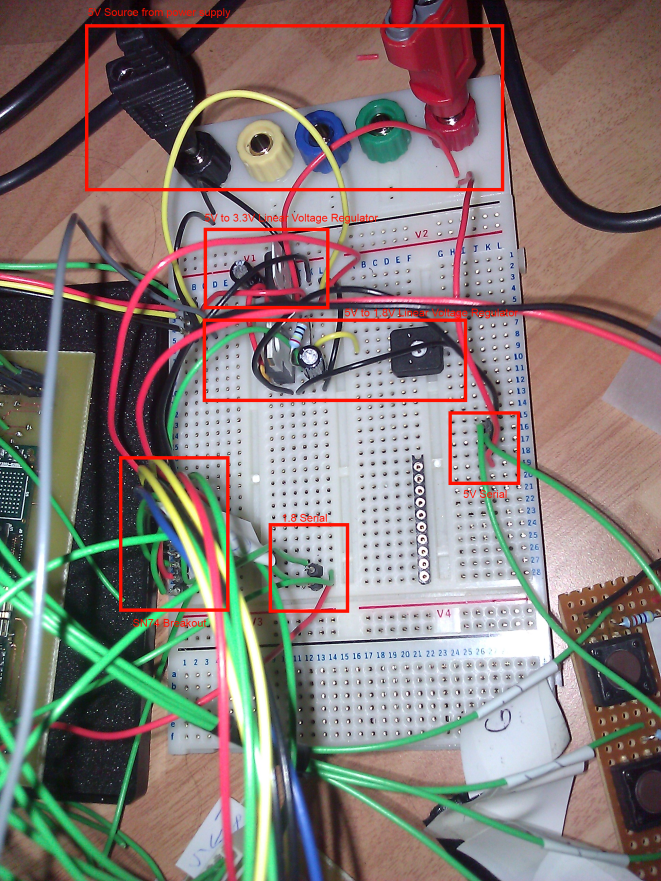
\includegraphics[scale=0.34]{images/breadboard.png}
		\caption{Breadboard Picture}\label{fig:breadboard}
	\end{figure}
	
	\section{Problems Encountered}
	\subsection{Team size and qualifications}
	Initially the team was constituted of four members, three electronic and 
	software engineering students and one electronic and electrical student.
	Due other work commitments the electronic and electrical student had to leave the
	team,  leaving only three members with the same degree. The teams 
	qualifications not being as diverse had some impact on the productivity of the
	hardware aspects of the project but, in contrast, allowed for fast development
	of the different software pieces. Another effect of the team being limited to only
	three members than the limitation of the work that could be done is that
	initially every team member had some allocated tasks and at the departure
	of the foruth member the tasks had to be reallocated and therefore modifying
	the schedule.

	\subsection{Printed Circuit Board}
	The software used to design the printed circuit board was PCB Editor from the
	OrCAD toolsuite. Even though most of the members had already some experience from
	second year with this software, the board that had to be designed for this
	project required more advanced knowledge, such as footprint design and track
	width adjustments. This lack of this knowledge meant that took a significant amount of time
	in the PCB design process.\\
	\\
	One issue was the design of the footprint for the board as the set of 
	footprints provided by the software is really limited.
	This meant that every footprint had to
	be designed from scratch.
	Unfortunately, some of them were incorrect and had to be redesigned during
	development. Due to
	some limitations of PCB editors all the footprints that required drill holes
	had to be edited in order to display the drill holes on the mask.\\
	\\
	Another main issue with the PCB was related to the components selected, some
	of them such as the Gumstix or the SN74 have a really small pin-to-pin spacing
	that makes them hard to be etched accurately on the board and makes them
	hard to solder. Thanks to Nick Scott the team have been able to use these
	components.

	\subsection{SPI Issues}
	The Serial Peripheral Interface (SPI) between the S08 and the gumstix caused
	the team some troubles and delayed the fabrication of the final board. The
	first issue that was trivial but not identified after a couple of hours was
	that the demo board for the S08 and the gumstix did not share a common ground
	and therefore the signal levels were incorrect.\\
	\\
	After this problem was resolved the SPI communication was working but not as
	expected and it was hard/impossible to identify when a byte was received
	between the value 0 and padding 0 to enable the transmission. After some
	analysis with a four channel oscilloscope, it was determined that the mode
	on the slave side was not the same on the master side leading to the
	perceived incorrect behaviour of the Chip Select line.

\chapter{Software System Design}
	\section{Introduction}
	The software for the dashboard also had to address some criteria. It essentially had to be able to 
	retrieve CAN data coming from the microprocessor and display this data in an understandable format
	to the driver. It had some other important functions to perform. In particular it was required 
	to act as a data logger as well. This means that it kept a record of all CAN packets received
	for the duration of the program.\\

	Several software systems have been implemented to support the system and 
	provide functionality. The following is a list of the developed software.
	
	\begin{itemize}
		\item LeadSoft Dashboard display application
		\item CAN to SPI converter and buffer for Freescale MC9S08DZ60
		\item Modified spi\_dev for SPI functionality on Linux
		\item Hardware keyboard driver over GPIO
		\item Leadsoft CAN logger reader
	\end{itemize}
	\section{Overview}
	\begin{figure}[H]
		\centering
		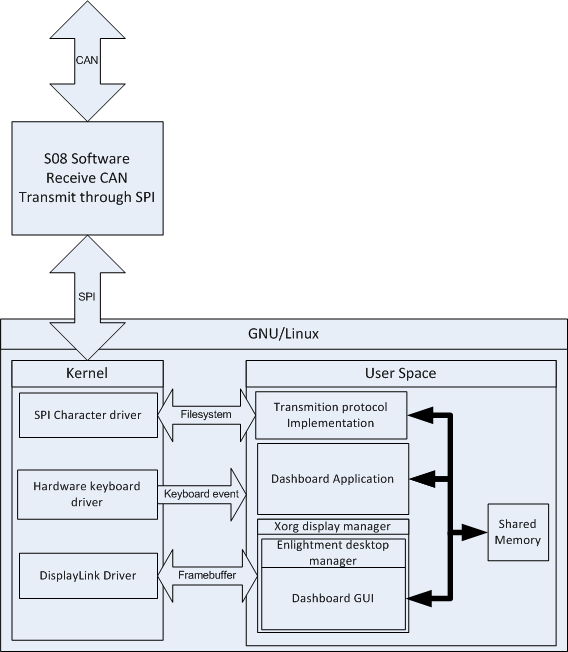
\includegraphics[scale=0.45]{images/software_diagram.png}
		\caption{Software Overview}\label{fig:software_diagram}
	\end{figure}

	\section{Boot Sequence}
	The boot sequence of the gumstix is fairly complicated as it consist of a two 
	stages boot loader; a first boot loader is used to load a second boot loader to
	finally load the required system. On the omap3503 the first boot loader is
	called X-Loader and is created by Texas Instrument, the second boot loader
	is ``Das Universal Bootloader'' commonly called U-Boot that loads the linux
	kernel into memory and starts it. Also U-Boot is used to configure the pin
	multiplexing on the micro processor.
	\begin{figure}[H]
		\centering
		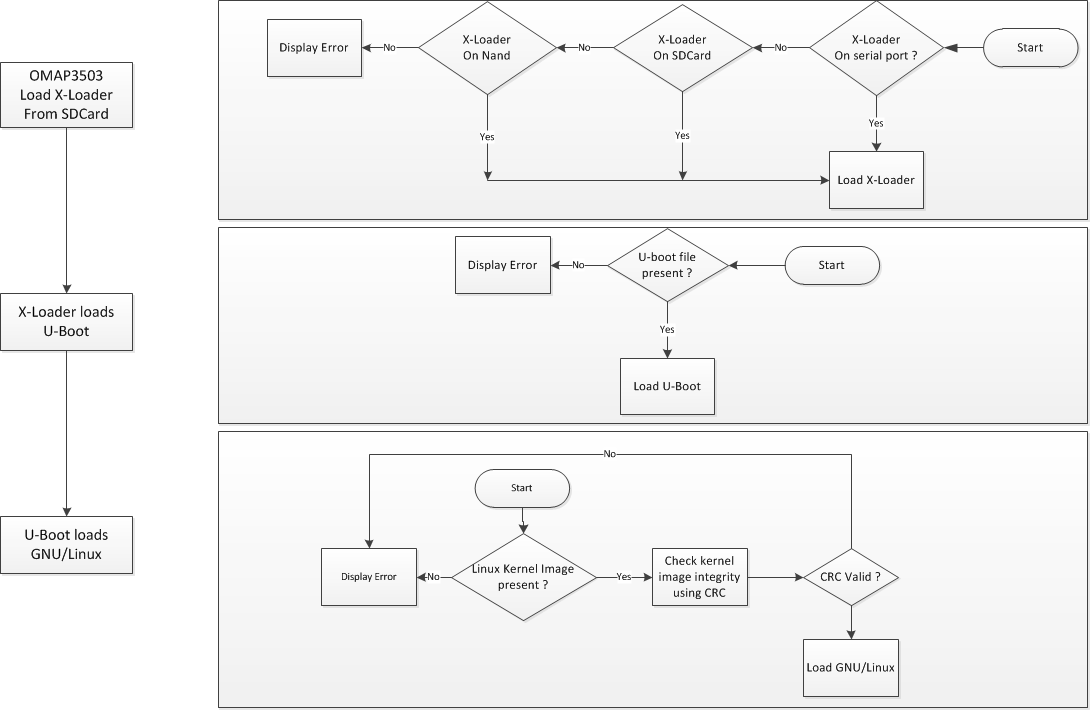
\includegraphics[scale=0.50]{images/boot.png}
		\caption{Boot Sequence}\label{fig:boot_diagram}
	\end{figure}

	\section{GNU/Linux}
	Three solutions were available for the team to base the software on
	\begin{itemize}
		\item Windows CE: Microsoft operating system for embedded devices that is not
		open source and provide support only for a few number of devices.
		\item No operating system: The team could have designed an application without
		using any operating system and compiling binaries directly for the omap3503.
		\item GNU/Linux: An open source operating system with a large community and a
		large number of already designed drivers.
	\end{itemize}

	The no operating system option has not been used because the overall developping time
	would have been too long as drivers for the SDCard (Secure Digital), USB stack, 
	Screen Drivers etc... should have been reimplemented and it was simply not
	possible to allocate so much ressources for the project. The overall
	improvement and efficiency of the final program did not worth the developping
	time.\\
	\\
	Windows CE has also not been used as the support by the gumstix community is
	really limited and most of the drivers that were required were either not stable
	enough for long term use or non existing such as the DisplayLink drivers.
	Another drawback of Windows CE is that a licence is required for every single
	device running the operating system.\\
	\\
	Therefore GNU/Linux has been used as it is the main operating system used by
	the gumstix community and has built-in support for DisplayLink, USB, CAN and
	most of what was required for the dashboard. However due to the large amount
	of drivers and possible configuration to suit the needs of a lot of embedded system
	the configuration of the kernel and the associated packages is not easy and
	requires a lot of compilation and configuration time.\\
	\\
	The following drivers and modules have been used
	\begin{itemize}
		\item UDLFB: USB DisplayLink Frame Buffer, to provide a frame buffer (file 
		used to store image to be displayed).
		\item SPIDEV: SPI User mode interface used for the MC9S08 communication.
		\item Kernel GPIO debouncing configuration to prevent the push button from 
		triggering multiple times.
	\end{itemize}
	
	The following software package have been used
	\begin{itemize}
		\item The Angström GNU/Linux distribution that is designed for embedded systems
		by removing unnecessary software packages not required on embedded devices.
		\item XOrg as display manager.
		\item GPE-DM (GNOME palmtop Environment) as desktop manager.
		\item Enlightenment user interface to provide an easy to use system.
		\item SDL (Simple DirectMedia Layer) to abstract the graphical operations.
	\end{itemize}

	More information about the Linux configuration is available on the Appendix.

	\section{Simple DirectMedia Layer (SDL)}
	
	\subsection {X11}
	X11 is a computer software system and network protocol. It aims to provide a standard set of 
	high level APIs for GUI development
	especially in networked computers (but is also heavily used on stand alone systems). It is ubiquitous because
	it creates a hardware abstraction layer for writing user interfaces, this allows applications written in X11 to be
	portable between different systems with different hardware, as long as these machines all support X11.
	
	Because the team had previous experience in Advanced Programming 3 course working the X11 display system,
	 initial intentions involved using X11 directly to create the  graphics system for the dashboard. 
	This would ideally run on Linux machine as a server 
	and render the graphic components to the screen as specified.\\

	This approach rapidly lost momentum as the team  realised that this could be a time consuming task.
	As an example, 
	the code snippet below identifies the steps required to render a window as full screen using the x11 display system.

\begin{lstlisting}
	
/* Step 1: inform the window manager that the window should have no borders */
Hints hint; // a struct for specifying prefrences
hints.flags = 2; // Specify that we would like to change the 
                 //windows decorationthat we're changing the window decorations.
hints.decorations = 0;  // 0 (false) means that there should be no decoration/borders for this window

property = XInternAtom(display,"_MOTIF_WM_HINTS",True);
XChangeProperty(display,window,property,property,32,PropModeReplace,(unsigned char *)&hints,5);
	
/* Step 2: resize the window to the size of the screen */
XF86VidModeSwitchToMode(display,defaultscreen,video_mode);
XF86VidModeSetViewPort(display,DefaultScreen,0,0);
XMoveResizeWindow(display,window,0,0,width,height);
XMapRaised(display,window);
XGrabPointer(display,window,True,0,GrabModeAsync,GrabModeAsync,window,0L,CurrentTime);
XGrabKeyboard(display,window,False,GrabModeAsync,GrabModeAsync,CurrentTime);
	
\end{lstlisting}

This is the minimum code required to setup the full screen capability of the X11 system.
From, it is not impossible to see how this could spiral into a more 
complex process for more complex functions. Putting into consideration that we would also
need to display graphics in the window, the team desired to look into other options available.\\

\subsection {Simple DirectMedia Layer}
SDL is a cross-platform, open source multimedia library written in C. It presents a simple
interface to various platforms, including graphics, sound, and input capabilities. Its primary aim is to provide
a uniform framework for accessing these. SDL itself is very simple;
it merely acts as a thin, cross-platform wrapper, providing support for a host of low level operations.\\

SDL is not far off from the X11 system in principle. Both systems abstract hardware
details from the programmer. On X11 platforms (such as linux), SDL uses Xlib to
communicate with the X11 system for graphics and events, i.e SDL acts as a layer of
abstraction above the X11 subsystem to provide graphics functionality for programs to application developers.
The diagram below illustrates the relationship between an X11 system, SDL, and a user GUI program.\\

\begin{figure}[H]
		\centering
		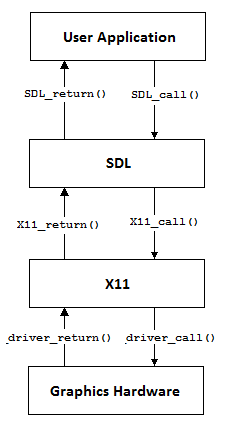
\includegraphics[scale=0.70]{images/several_layers.png}
		\caption{Relationship between SDL, X11 and Hardware}\label{fig:several_layers_diagram}
	\end{figure}

By providing this layer of abstraction, SDL makes GUI programming a lot easier compared to directly 
programming with the X11 display system. For instance, to enable the full screen using SDL libraries, one would 
simply the need to add the {\bf SDL\_FULLSCREEN} flag as a parameter to {\bf SDL\_SetVideoMode} call as seen below:

\begin{lstlisting}
screen = SDL_SetVideoMode(800, 480, 24, SDL_SWSURFACE | SDL_DOUBLEBUF | SDL_FULLSCREEN);
\end{lstlisting}

This is obviously a lot easier to comprehend in the limited time that we had for the project.
Other advantages of using SDL would be that:
	\begin{itemize}
		\item if offers its own thread libraries, along with semaphores, mutexes and other concurrency handlers
		\item it allows images to be displayed in a presentable way and with minimal effort
		\item it offers library functions which allow events to be captured and triggered easily from sources such as the keyboard and mouse
		\item it offers library functions for  audio, file access, and  timing.
	\end{itemize}


For these reasons, the team unanimously decided to make use of the SDL libraries for the GUI development.		
				
	\section{LEAD Software}

	\subsection{GUI design}
	The GUI was designed to be intuitive to use. Since the product was being designed
	for a vehicle, it should provide minimum distraction to the driver under normal operating
	circumstances, but provide a quick response when the driver wishes to know certain bits 
	of information. To this end, much time and effort was put into the design of the user interface.

	The team categorised each of the displayable items according to their level of 
	importance to the driver. The items that ranked the highest stayed closer to 
	the centre of the screen where the driver could glance at with minimal effort. 
	Items and their prioritisation are listed below:

	\begin{itemize}
		\item car speed - highest priority
		\item gear number - high priority
		\item rpm - high priority
		\item engine temperature - medium priority
		\item oil temperature warning signal - medium priority
		\item coolant temperature warning signal - medium priority
		\item oil temperature - low priority
		\item coolant temperature - low priority
	\end{itemize}

	Each of these sources would have its own on screen 'Widget'. The widgets in the GUI were 
	categorised according to the roles they play. The four main categories are discussed below.

	
	\subsubsection{Labels}
		
	Labels are used to display strings of texts to the screen. They were grouped into 
	fixed and variable labels. \\
			
	Fixed labels do not change their value throughtout the programs duration
	as such they do not need to be refreshed or re-written to the screen. Example of a fixed label
	is the "ENGINE TEMP" and "GEAR" texts. \\
			
	Variable labels do not change their values frequently. As such, they need to be refreshed at a constant rate.
	Example of such labels include the engine temperature value and the speed value.
			
	\subsubsection{Icons}
			
	Icons are used to display images/symbols that can be easily noticed by the driver. 
	Each icon has two states attributed to it. These are {\bf state\_on} and {\bf state\_off}. Both states have images associated 
	with them.
	By  switching between both states, icons have the ability to blink. 
	Examples of icons used include the coolant temperature warning light and oil temperature warning lights.
			
	\subsubsection{Bar Graphs}
		
	Bar graphs are used to illustrate values in a graph format. This is easy to interpret by the driver
	as he/she can view the information instantaneously and have an estimate of the value. The Bar graphs 
	work by storing two images. These images represent its full state and its empty state. A fraction of the full image that 
	corresponds to the value to be represented is displayed. The rest of the graph is filled with the empty graph image.
	As well as direction, maximum values of graphs can be set by the users.
			
			
	\subsubsection{Graph Movement}
			
	\begin{itemize}
	\item Horizontal Bar Movement: \\
	 The horizontal movement of the graph could be from left to right or right to left.
	 This is specified in the direction variable.If the direction is specified as left
	 to right then a portion of the full image is placed on the display. The remaining
	 portion allocated to the graph is filled with the empty image. An example of a graph
	 widget that moves horizontally is the {\bf engine rev} bar graph as shown below.
				
	\begin{figure}[H]
	\centering
	
\includegraphics[scale=0.80]{images/rpm_graph_full.png}
	\caption{Diagram showing a Full horizontal bar graph}\label{fig:rpm_graph_full_diagram}
	\end{figure}
	
	\begin{figure}[H]
	\centering
	
\includegraphics[scale=0.80]{images/rpm_graph_empty.png}
	\caption{Diagram showing an empty horizontal bar graph}\label{fig:rpm_graph_empty_diagram}
	\end{figure}
				
	For example, given a maximum graph value of 100, if the value being read from the CAN bus is 30. Then the portion of the
	full graph to be displayed is calulated as:
	
	\begin{center}			
	\begin{equation}
	\aligned
	width\_to\_display &= \frac{30}{100} \times width\_of\_full\_image
	\endaligned
	\end{equation}				
	
	Thus for a given maximum graph value M and arbitrary CAN value V:
	
	\begin{equation}
	\aligned
	width\_to\_display &= \frac{V}{M} \times width\_of\_full\_image
	\endaligned
	\end{equation}				
	\end{center}
				
	\item Vertical Graph movement: \\
	The vertical graph is capable of moving up to down or down to up as 
	specified by the direction parameter. It differs only slightly from the horizontal
	bar graphs. All that is adjusted in this case is the fraction of the total height 
	of the full image being displayed. An example of a graph widget configured for vertical
	motion is the {\bf fuel level} bar graph shown below.\\
	
	\begin{figure}[ht]
	\begin{minipage}[b]{0.5\linewidth}
	\centering
	
\includegraphics[scale=0.50]{images/fuel_empty.png}
	\caption{An empty vertical bar graph}
	\label{fig:figure1}
	\end{minipage}
	\hspace{0.5cm}
	\begin{minipage}[b]{0.5\linewidth}
	\centering
	
\includegraphics[scale=0.50]{images/fuel_full.png}
	\caption{A full vertical bar graph}
	\label{fig:figure2}
	\end{minipage}
	\end{figure}		
	
	
	For example, given a maximum graph value of 100, if the value being read 
	from the CAN bus is 45. Then the portion of the vertical graph to be displayed is calculated as:
					
	\begin{center}			
	\begin{equation}
	\aligned
	height\_to\_display &= \frac{45}{100} \times height\_of\_full\_image
	\endaligned
	\end{equation}				
	
	Thus for a given maximum graph value M and arbitrary CAN value V:
	
	\begin{equation}
	\aligned
	height\_to\_display &= \frac{V}{M} \times height\_of\_full\_image
	\endaligned
	\end{equation}				
	\end{center}					
					
	\item Optimisation:\\
	In both movements forms discussed above, there would be an overhead of laying the same image
	in the same location repeatedly. In order to optimise performance and save redundant screen manipulation time,
	the code was changed so that only portions of the screen where a change was needed were changed.
				
	For instance if the current graph value was 30\% of the maximum
	
		\begin{figure}[H]
	\centering
	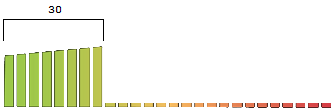
\includegraphics[scale=0.80]{images/rpm_30.png}
	\caption{}\label{fig: rpm 30}
	\end{figure}

				
	and the new value was 50\%, to be representd as: 
	
	\begin{figure}[H]
	\centering
	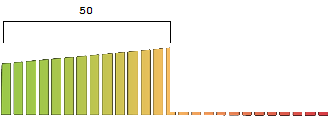
\includegraphics[scale=0.80]{images/rpm_50.png}
	\caption{ }\label{fig:rpm 50}
	\end{figure}
	
	then only the additional 20\% would be added.
				
	\begin{figure}[H]
	\centering
	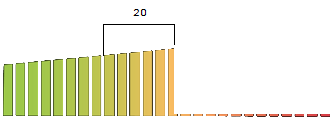
\includegraphics[scale=0.80]{images/rpm_combo.png}
	\caption{ }\label{fig:rpm combo}
	\end{figure}
			
				
	This is a better approach than overlaying the screen with the new 50\% data, which
	unnecessarily overwrites the previous value.
	Only the area of the graph marked by the 20\% would be updated to the display.
	This is a better approach than overlaying the screen with the new 50\% data because doing so involves
	writing to screen the exact image pattern that was already there. This substantially reduced the 
	amount of time needed for one cycle of refreshing the display. The time cut is very useful because it allows more 
	time for data processing, i.e processing of the recieved CAN packets. 
	\end{itemize}
	\section {Application Design}
	
	
	In designing the application, the team split the application into its component functionalities. 
	These are:
	
	\begin{itemize}
	\item Drawing the display items to the screen
	\item Reading and acting on user unput
	\item Reading data from the SPI interface
	\end{itemize}
	

	
	\subsubsection{Main Thread}
		The function of the main thread is to initialise all other variables that are needed for the GUI to be displayed.
		It also sets up the SPI subsystem for reading  and writing operations by another thread.
		After all setting up and initilaisation is done, the main thread functions as the screen updating thread
		for the duration of the program. It draws to the screen only those pixel segments that have changed since the last screen draw.
		
	\subsubsection{Reading User input}
		A different thread reads the user's input. This thread is primarily used to navigate around the configuration and diagnostic 
		menu. Another important function of the read user input thread is to send gear up and gear down messages to the CAN network.
		The thread waits until one of the four pushbuttons is pressed.
		
	\subsubsection{Reading from SPI}		
		A third and final thread is used to read data from the SPI. The thread uses the SPI protocol the team defined, to 
		simultaneously read from and write byte sequences to the microcontroller. This full duplex transfer is very useful
		as it ensures that there is no time wasted in issuing a separate write command.\\
	
	The image below best illustrates the flow of control from the start to end of the program.
	
	\begin{figure}[H]
	\centering
	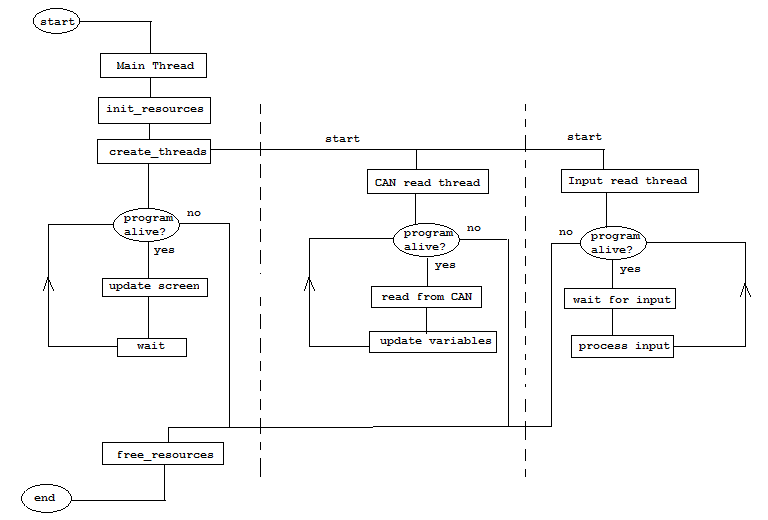
\includegraphics[scale=0.80]{images/program_arch.png}
	\caption{Flow control of the LEADsoft dashboard display program}\label{fig:program architecture}
	\end{figure}
	
	
	\subsection {Menu}
		
		The menu system can be accessed by using the right arrow key. This stops the updating of CAN packets to screen and
		opens a menu window. The user has a choice of configuring the warning levels for CAN data or viewing the diagnostics.
		The various options can be assessed by using the arrow keys up and down. In the menu window, a user can:
		
			
	\begin{itemize}
	\item configure variables for warning levels
	\item enter diagnostics mode to view packets received
	\item quit the program
	\item shut the system down
	\end{itemize}
	
		
	\subsubsection{Diagnostic}
		
		The diagnostics is a simple human readable window that allows a user to view the CAN packets receieved. The diagnostics 
		was implemented by reading logged CAN data and displaying it. When the user wishes to scroll up, a portion of the log file 
		representing the portion of data that the users wishes to view is processed and displayed.
		
	\subsubsection {Configuration}
	\label{diag_menu}
		
		In the configuration mode, the user can make a host of changes to system. In particular a user can decide what values
		to associate with the warning levels for specific CAN data. Configurable items include:
			
	\begin{itemize}
	\item Speed source: road speed, wheel speed or GPS speed.
	\item RPM bar graph maximum value.
	\item Engine temperature warning level.
	\item Coolant temperature warning level.
	\item Fuel low flashing indicator warning level.
	\end{itemize}
		
	Once the data is set, it is saved to a file. So the new warning values are used until 
	such time as new values are established.

	\subsection{CAN Logger}
	A CAN packet logger has been written as part of the LEAD Software package. This
	logs every CAN packet received by the Gumstix to a file. However, this file is not
	human readable, and a standalone application has been developed to view the log
	file contents. Live CAN data can be viewed on the Gumstix through the dashboard
	diagnostic menu. (see \ref{diag_menu}).
	
	\subsection{SPI driver}
	
	The team developed a custom linux SPI driver for reading and writing to the CAN data
	to the microntroller. In its initial phase, arbitrary values were given for the SPI configuration.
	These were:
		 
	\begin{itemize}
	\item spi mode
	\item spi bit : specifies number of bits per byte of SPI transfer
	\item spi speed : speed in hertz
	\item spi delay
	\end{itemize}
	
	However, due to some bugs in the driver, frequent kernel crashes occured. 
	As a result, the team decided to use standard SPIdev driver.
		
	\subsubsection {SPIDEV}
	SPIdev is the standard built-in SPI device driver for linux systems. It has full duplex capability.
	It works by establishing an SPI connection with a slave device and creating a absract file stream that
	represents the established connection. Subsequent reads and writes to the file are then transfered to the SPI
	slave.
		
	To get SPIdev working, the linux operating system had to be configured and recompiled. This seemed to be the solution
	and a better alternative to writing a custom driver from scratch.\\
	 
	The team also developed an SPI protocol for reading and writing CAN packets between the gumstix and the
	microcontroller. See SPI protocol section.
	 
	\subsection{Software problems}
	\subsubsection{GUI Flickering}
	 During the GUI testing phase, the team noticed that the response of the update thread was slow.
	 Graphs and other widgets seemed to blink when their values changed.
	 
	 The solution to this was to use double buffering. With double buffering, graphic objects are
	 drawn into a special memory banks the size  and later drawn to screen on request. So the screen 
				
	\section{Freescale MC9S08 Programming}
	The primary purpose of the Freescale S08 microcontroller is to provide CAN
	functionality to the system. It should also store data in a custom packet
	format for transmission over SPI. SPI data should be buffered, and the S08
	should respond to command packets from the SPI master (the Gumstix). An
	indication of data flow is given below.\\
	
	CAN data is received via an interrupt, which extracts the CAN data and
	creates a packet of the SPI packet format which is put in an SPI buffer
	for queued transmission. Meanwhile when the Gumstix is running and
	providing an SPI clock, data is transmitted a byte at a time between the
	devices.\\
	
	For CAN data, SPI packet data has a minimum size of 3 bytes (CAN\_DLC of 0)
	and a maximum size
	of 11 bytes (CAN\_DLC of 8). Since data needs to be transmitted one byte at
	a time, the data must be split into a stream of bytes, instead of sending
	one field at a time. The byte ordering is as follows.
	
	\begin{itemize}
		\item Byte 1: bits [7:6] Status bits - 01 for CAN 
		\item Byte 1: bits [5:0] top 6 bits of CAN11 ID [10:5]
		\item Byte 2: bits [7:3] bottom 5 bits of CAN11 ID [4:0]
		\item Byte 3: bits [3:0] 4 bit CAN Data Length Code
	\end{itemize}
	
	\subsection{Example CAN to SPI conversion}
	To illustrate the SPI protocol and packet construction, the following
	is an example of a CAN packet being received bearing the information
	of a gear position of 2.
	The CAN packet data is:
	
	\begin{itemize}
		\item CAN ID: 0x1A0 - 0b001 1010 0000 
		\item CAN DLC: 1 
		\item Data: 2 (The gear position)
	\end{itemize}
	
	This packet will be translated by the CAN Interrupt service routine on
	the microcontroller to:
			
	\begin{itemize}
		\item Byte 1: 0100 1101 - 4D (Status 01 = CAN11 packet)
		\item Byte 2: 0000 0000 - 00
		\item Byte 3: 0000 0001 - 01 (DLC = 1)
		\item Byte 4: 0000 0010 - 02 (Data = 2)
	\end{itemize}
	
	This is transmitted over SPI a byte at a time, and reassembled into individual
	fields, discarding the Status bits.
	Since the DLC is read as one byte, the SPI receiver can calculate from that
	how many more bytes are going to arrive before there could be a 
	new packet (i.e. status code) to process.

	\section{SPI protocol}
	\label{sec:spi_proto}
	It is assumed in this protocol that the data would not be corrupted
	during the SPI communication therefore this protocol does not define
	integrity checks and error correction. It is also assumed that when the
	slave select line is de-asserted the SPI buffers in both the client and
	server sides are flushed, this is to prevents unknown state and possible
	synchronisation issues.	 

		\subsection{Packet structure}
			\subsubsection{Global Structure}
				\begin{tikztimingtable}
				SIZE	 & GN 2D{2} 6D{VARIABLE} GN \\
				PACKET	 & GN 2D{OP} 6D{DATA} GN \\
				\end{tikztimingtable}

				\begin{table}[h]
				\centering
				\caption{Operation codes and values}
				\begin{tabular}{| l | c | c |}
				\hline
				Operation & Value(\#2) & Description \\
				\hline\hline
				CMD	& 00 & Command Packet \\
				D11 & 01 & 11bits identifier CAN packet \\
				D29 & 10 & 29bits identifier CAN packet \\
				\hline
				\end{tabular}
				\label{tab:global_struct}
				\end{table}

				\indent Every packet must have a two bits packet identifier to indicate
				the type of the outgoing data. The table \ref{tab:global_struct}
				contains the command codes used in this protocol to send command
				messages and CAN packet with an identifier of length 11 and 29.

			\subsubsection{CMD Packet}
				\begin{tikztimingtable}
				SIZE	 & GN 2D{2} 6D{6} GN \\
				PACKET	 & GN 2D{CMD} 6D{CMD\_CODE} GN \\
				\end{tikztimingtable}

				\begin{table}[h]
				\centering
				\caption{Command codes and values}
				\begin{tabular}{| l | c | c |}
				\hline
				Command & Value(\#10) & Description \\
				\hline\hline
				CMD\_NULL & 0 & Do nothing \\
				CMD\_START & 1 & Start data transfer \\
				CMD\_STOP & 2 & Stop data transfer \\
				CMD\_EOS & 3 & End of stream \\
				\hline
				\end{tabular}
				\label{tab:cmd_codes}
				\end{table}

				\indent The command packet is used to initiate and indicate the current
				status of the transmission. The list of available commands can be seen
				in the Table \ref{tab:cmd_codes}. The number of possible commands is
				limited to 64 as the command field is 6 bits long.

			\subsubsection{DATA11 Packet}
				\begin{tikztimingtable}
				SIZE	 & GN 2D{2} 11D{11} 4D{4} 8D{0..64} GN \\
				PACKET	 & GN 2D{D11} 11D{CAN\_ID} 4D{DLC} 8D{DATA} GN \\
				\end{tikztimingtable}

				\indent The DATA11 packet is used to transfer a CAN packet where the
				CAN identifier is 11 bits long, the DLC value should be specified
				precisely or the transmission will go out of sync as the amount of
				data read and the data in the transmit buffer will be different.

			\subsubsection{DATA29 Packet}
				\begin{tikztimingtable}
				SIZE	 & GN 2D{2} 29D{29} 4D{4} 8D{0..64} GN \\
				PACKET	 & GN 2D{D29} 29D{CAN\_ID} 4D{DLC} 8D{DATA} GN \\
				\end{tikztimingtable}

				\indent The DATA29 is similar to the DATA11 packet however it is used
				to transfer the CAN packet with a 29 bits long identifier.

		\subsection{Transfer}
			\subsubsection{Read one packet}
				\begin{tikztimingtable}
				CLK		& 	68{c} \\
				SS 		& 	h 33L h \\
				MISO	& 	x 8U 25D{PACKET} x \\
				MOSI 	& 	x 8D{CMD\_START} 8D{CMD\_STOP} 17U x\\
				\end{tikztimingtable}

				\indent A single packet can be read by sending the start and stop 
				packet
				back to back the master will have to ensure that it finishes reading
				the packet before de-asserting the slave select line.

			\subsubsection{Read all packets}
				\begin{tikztimingtable}
				CLK		& 114{c}\\
				SS		& h 56L h\\
				MISO	& x 8U 10D{PACKET} 10D{PACKET} 10D{PACKET} 8D{CMD\_EOS} 
				10D{CMD\_NULL} x\\
				MOSI	& x 8D{CMD\_START} 8D{CMD\_NULL} 8D{CMD\_NULL} 8D{CMD\_NULL} 
				8D{CMD\_NULL} 8D{CMD\_NULL} 8D{CMD\_STOP} x\\
				\end{tikztimingtable}

			\subsubsection{Read and write}
				\begin{tikztimingtable}
				CLK		& 113{c}\\
				SS		& h 56L h\\
				MISO	& x 8U 10D{PACKET} 10D{PACKET} 10D{PACKET} 8D{CMD\_EOS} 10D{CMD\_NULL}x\\
				MOSI	& x 8D{CMD\_START} 10D{PACKET} 10D{PACKET} 10D{PACKET} 
				10D{PACKET} 8D{CMD\_STOP}x\\
				\end{tikztimingtable}
		
	\section{Problems Encountered}
		

\chapter{Testing}
	\section{CAN Testing}
		\subsection{Mircocontroller CAN Testing}
			To test the CAN receive code that was written for the S08 Microcontroller,
			The team used a given DEMO board which contained the same S08 controller for
			as was planned for the final board, an MC9S08DZ60.
			This was used in conjunction with an MC9S12XEP100 DEMO board to test CAN.
			A program was supplied by the UGRacing team, which could 
			read any CAN received packets and generate simulated CAN 
			packets for transmission over the S12 MSCAN module. This was flashed to the S12
			demo board, which allowed testing of the CAN interrupt on the S08 and 
			was able to test the S08 CAN transmit code once SPI had 
			been implemented.
	
	
			%Include info about using S12 as test input, debug on S08 etc.
		\subsection{Linux CAN Testing}
			Whilst CAN and SPI development was ongoing on the S08, the team needed to
			test CAN functionality of the GUI. Rather than wait until progress on the S08 had
			been made, the team created an application which could generate dummy CAN packets using a virtual
			CAN connection.
			This used socketCAN in the dashboard application. SocketCAN is an API which allows CAN 
			connections to be implemented in the same manner as normal connections using the Berkeley
			sockets API. It essentially creates a new network device which has a connection which can be opened
			closed, read from and written to. 
			This proved useful, as the CAN-USB devices worked over socketCAN, so since the application worked
			with socketCAN, the SPI through S08 approach could be switched out for a CAN-USB module at any time.
			%dummy CAN program on socket CAN test
	\section{SPI Testing}
		The SPI protocol (see \ref{sec:spi_proto}), was to be implemented as a full duplex 
		protocol on both ends. Initial testing though, was half duplex. With the data
		going one way, and NULL values going the other way.
		First tests with the spi-dev driver used a test program in the S08, which sent
		a series of incrementing values. Initial testing showed that these values were
		being successfully received. However, spurious 0 values between data values was
		a concern. However, this was solved after the realisation that there was no
		common ground between the Gumstix and the DEMO S08. Once a common ground was 
		established, the data output was as expected.\\
		Another SPI test involved the selection of an SPI Clock Mode to match the
		protocol. These are specified in the master and slave, so that they both
		know when to transmit data over the SPI line based on the $\overline{SS}$
		line.
		To check that our protocol was working as expected an oscilloscope was attached
		to the SPI lines and traces taken.
		A trace showing a gear change of 2 is shown below.
		\begin{figure}[H]
		\centering
		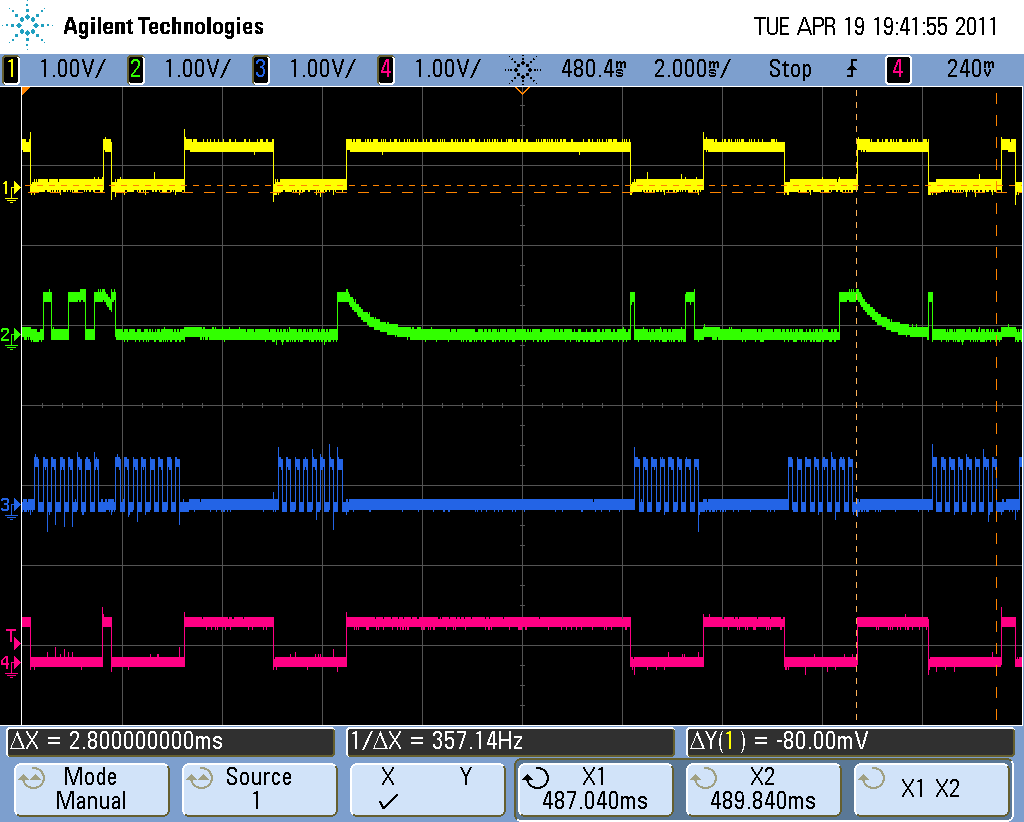
\includegraphics[scale=0.25]{images/GearChange2.png}
		\caption{SPI gear change}\label{fig:program architecture}
		\end{figure}
		Here we can see the 4 lines, MISO, MOSI, Clock and $\overline{SS}$ 
		%Dan's driver
		%spi_dev driver
		%Scoping the lines
		%Fixes and final implementation
	\section{Software Testing}
		\subsection{Off chip Testing}
			%Test and developm off the gumstix on linux
			%making sure that code compiles before porting
		\subsection{Gumstix on chip testing}
			Before Testing on the Gumstix could begin, a temporary power supply was
			assembled on a bread board to provide 3V and 1.8V from a 5V bench
			power supply. The lines on the Gumstix breakout board (see 
			\ref{gumstix_breakout_diagram}) were tested to ensure that the correct 
			voltages were present, before docking the Gumstix to the soldered dock
			connectors. 
			%Initial switch on and interaction over TTY serial connection
			%Display driver testing
			%kernel compilations
			%lightening the Linux distro
			%final solution
			%test programs, use USB hub etc
			%SDL intergration
			%SDL testing on Gumstix

\chapter{Possible Improvements}
	\section{USB Hub Functionality}
	Although at present a USB hub can be plugged into the USB host on the device to
	provide extra USB devices, a USB host on board would allow for multiple USB
	devices to be added, at the expense of space on the board for the USB ports.
	
	\section{Package Size}
	The final board turned out to be larger than expected because all of the 
	components were placed on the same side of the board. It could have been made into a smaller
	package by having devices on both sides of the board. 
	
	\section{CAN Logger Efficiency}
	The CAN logger currently logs all received CAN packets with 8 bytes of data, ignoring the DLC value.
	Although this allowed for easier parsing of the log file, (as the sizes of every packet were the same
	so the file pointer had a constant increment to get to the head of packets) it did waste storage,
	and a more efficient solution could have been made

\chapter{Conclusion}
 This project provided us with a great challenge and a potential for being creative in our approach to our solution. 
 The planned product would show our ability to deal with hardware design issues, while giving us the 
 ability to create a software solution in a familiar and powerful GNU/Linux environment. The design process increased our
 ability to use packages such as OrCAD Capture and PCB Designer, and the importance of getting the design correct.
 A great deal was also learned about communication standards such as CAN and SPI, and being able to implement these
 correctly was satisfying task.
 
 Teamwork was also an essential part of the effort, the ability to co-ordinate efforts and select people with the most
 experience and ability allowed us to ensure that we could deliver a quality product.
 
 The project was not without hindrances, and there were many times when, had the team not been careful and 
 thorough, we could have destroyed an expensive and essential piece of hardware, hence rendering our efforts
 useless. Due to our careful approach though, this was not a problem, and the Gumstix provided a great platform
 for development.\\
 From PCB design, to custom protocol specification, learning new programming interfaces and using libraries such as SDL.
  The teams approach to this problem has taken into consideration all of our collective skills gained throughout
studying our degree, to deliver a solution that is fast, efficient, flexible and can be easily extended. We believe that 
we have 
ultimately put the power of Linux into the hands of the driver.

\appendix
\chapter{Circuit Diagrams}
\label{app:circuit_diagrams}
	\section{Gumstix Breakout Board}
	\label{gumstix_breakout_diagram}
	\begin{figure}[H]
		\centering
		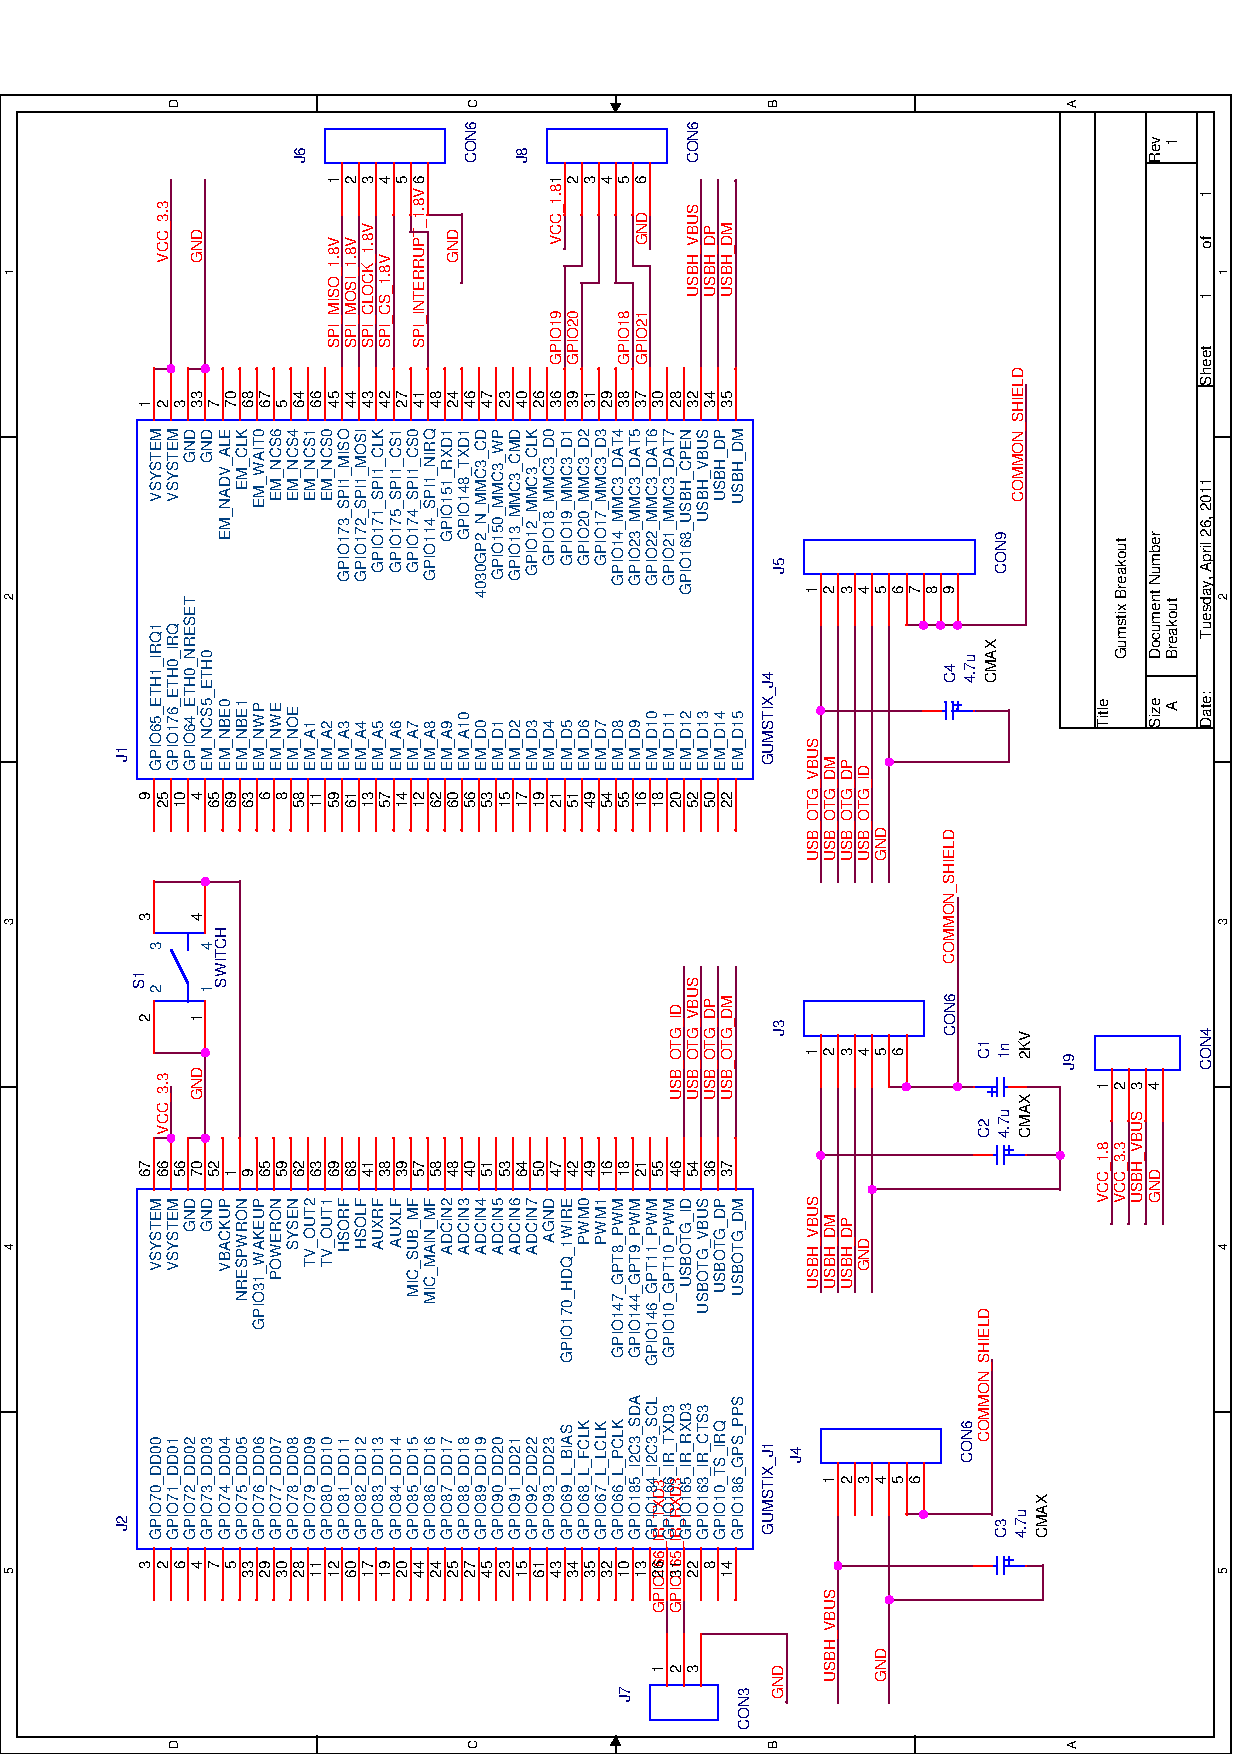
\includegraphics[scale=0.50]{images/breakout.png}
		\caption{Breakout Board}\label{fig:breakout_board}
	\end{figure}
	
	\section{SN74 breakout board}
	\label{SN74_breakout_diagram}
	\begin{figure}[H]
		\centering
		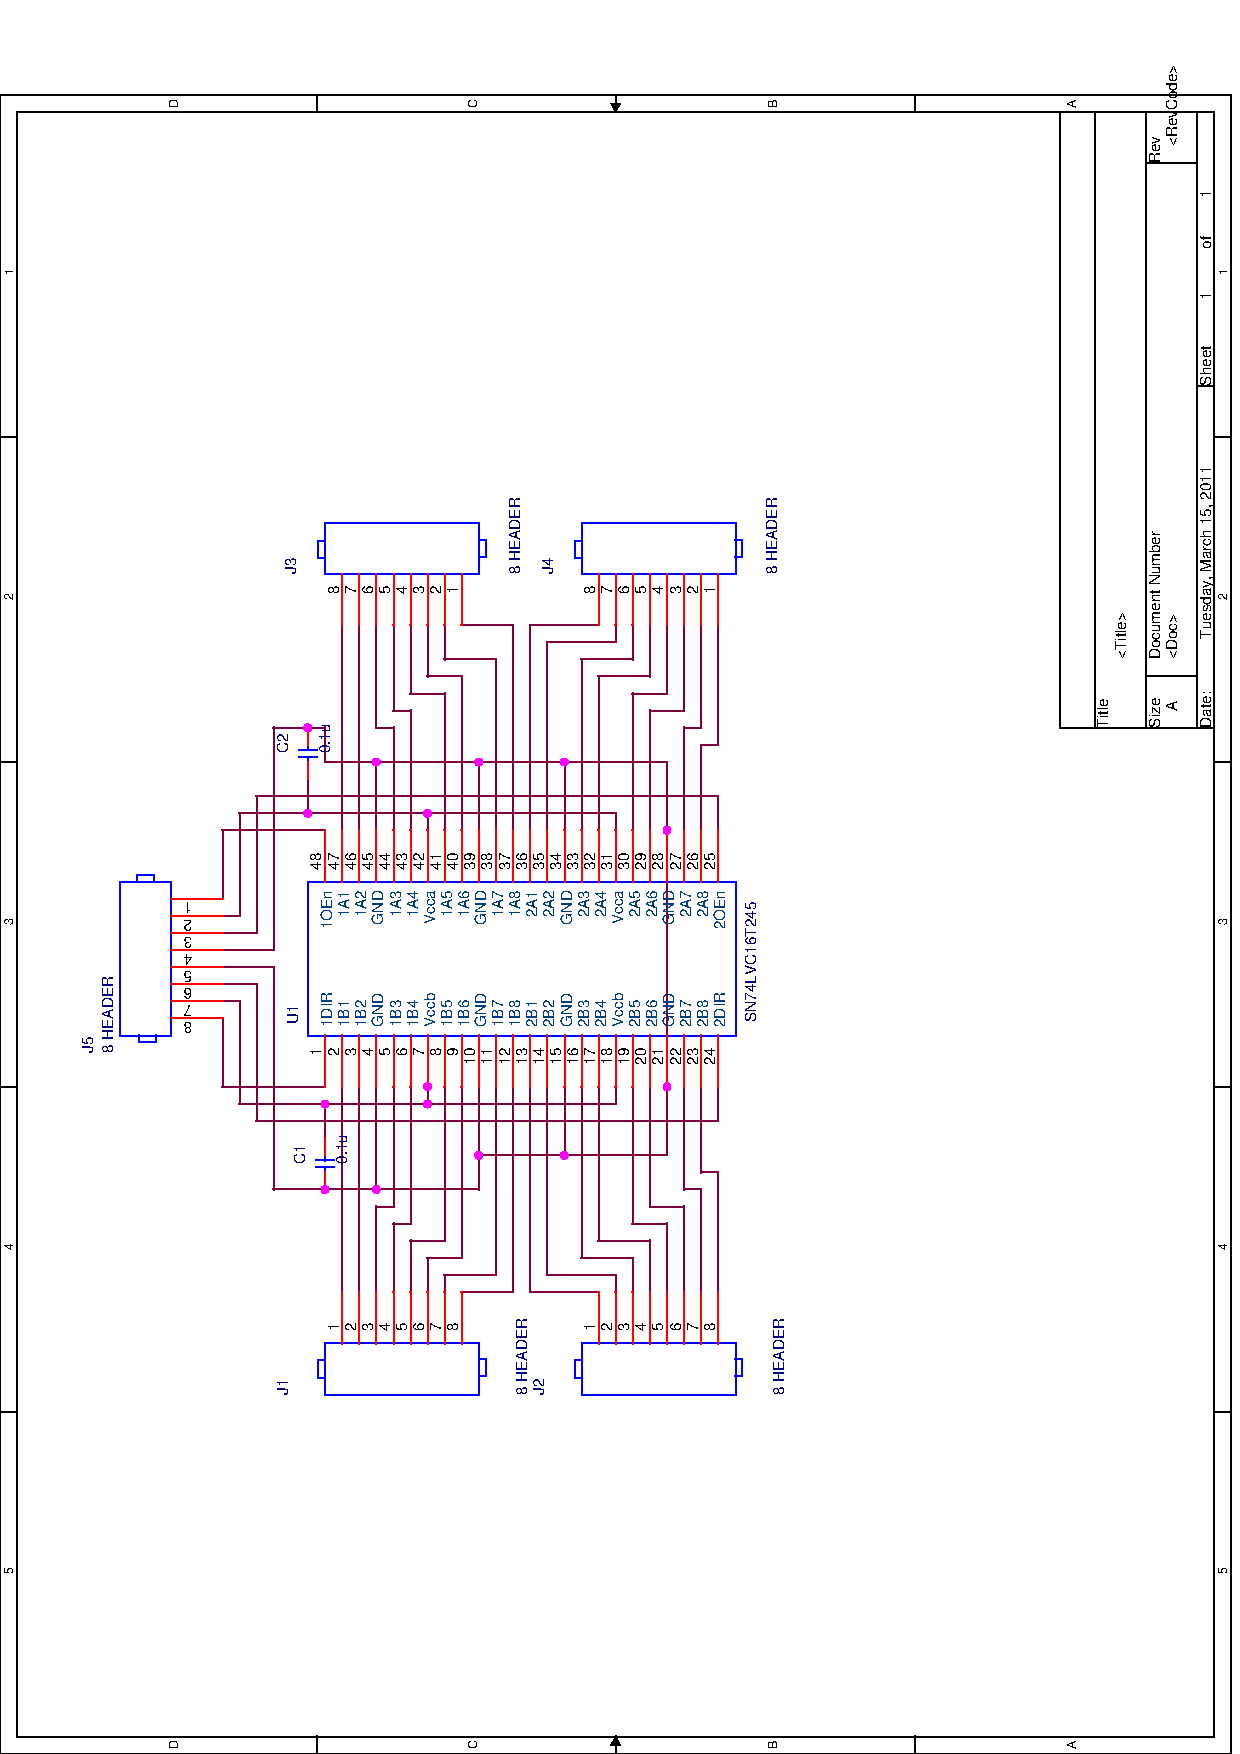
\includegraphics[scale=0.50]{images/sn74.png}
		\caption{SN74 Board}\label{fig:sn74_board}
	\end{figure}
	
	\section{Final Board}
	\label{final_board_diagram}

	\begin{figure}[H]
		\centering
		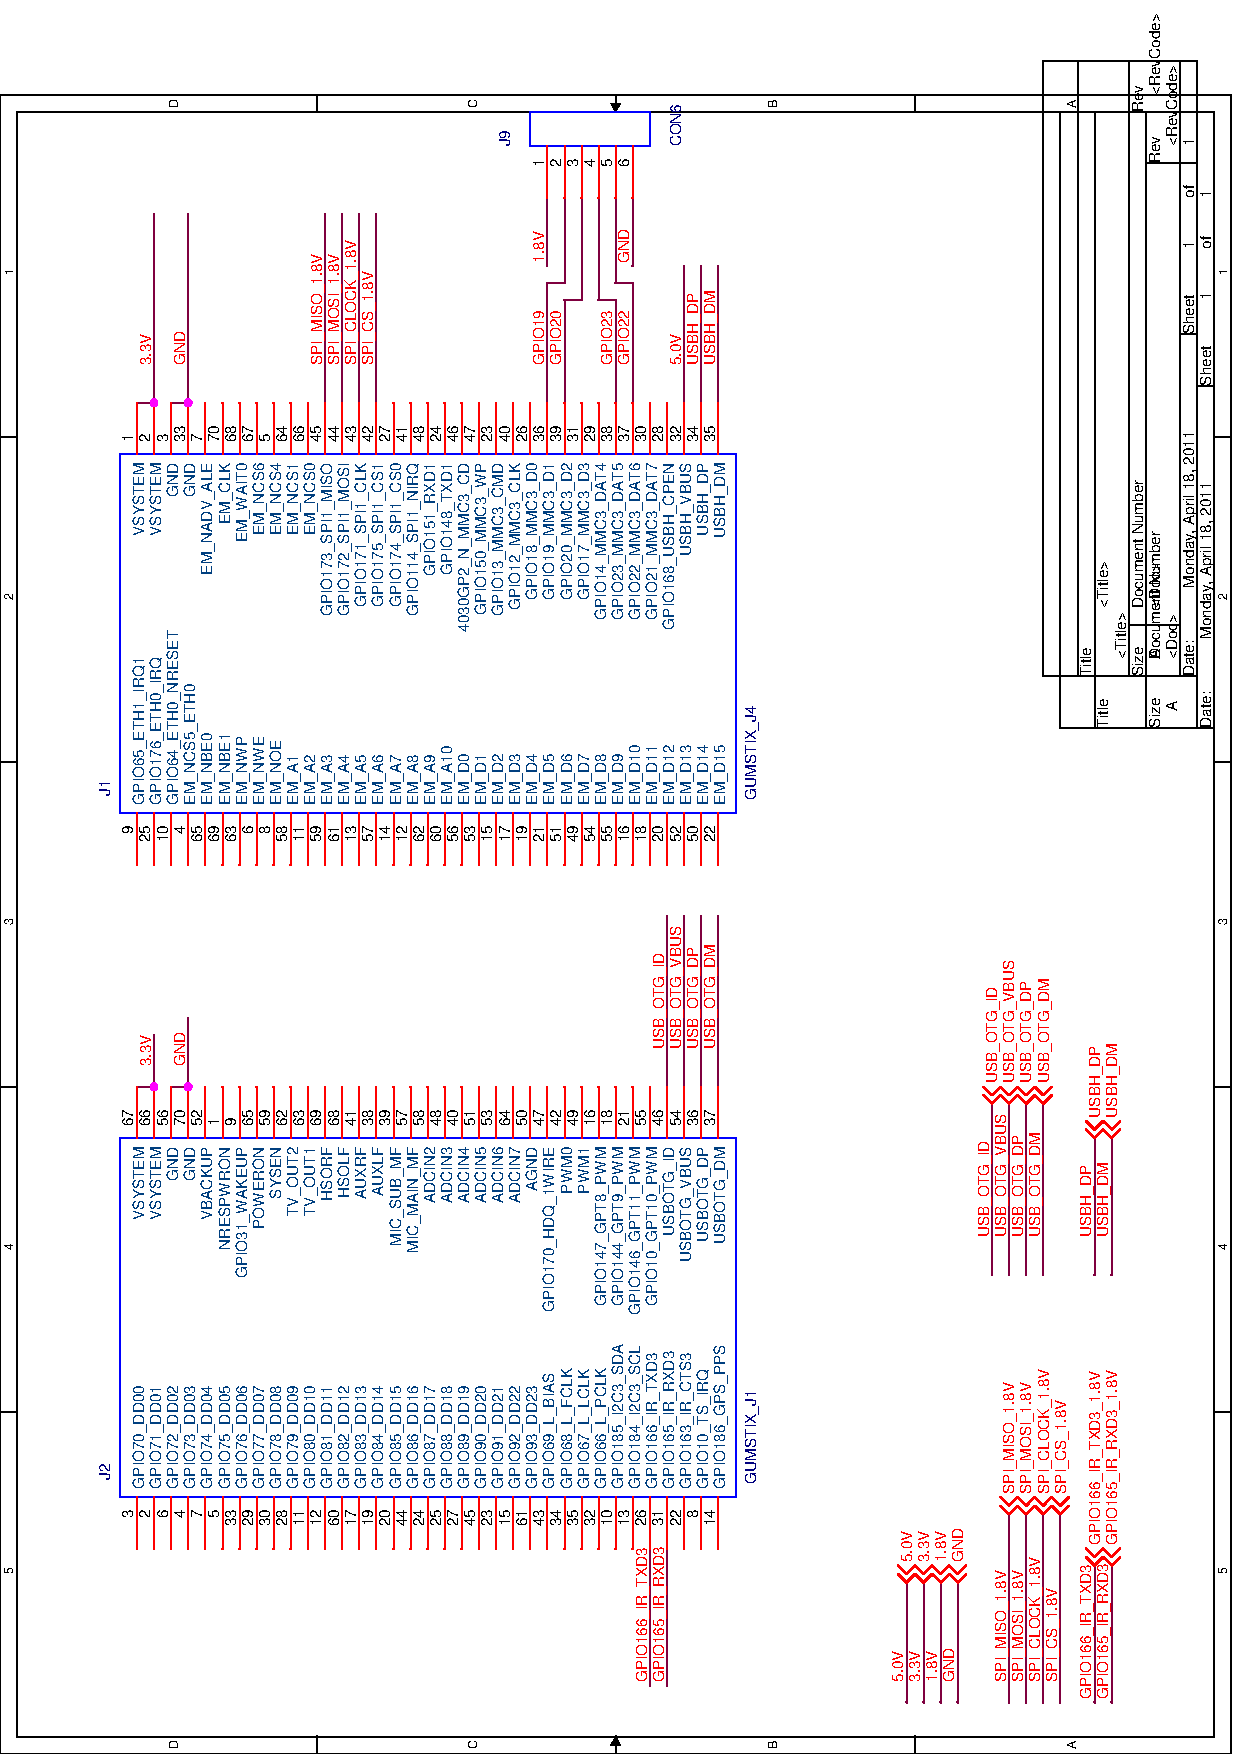
\includegraphics[scale=0.50]{images/final_gumstix.png}
		\caption{Gumstix Section}\label{fig:finalgumstix_board}
	\end{figure}

	\begin{figure}[H]
		\centering
		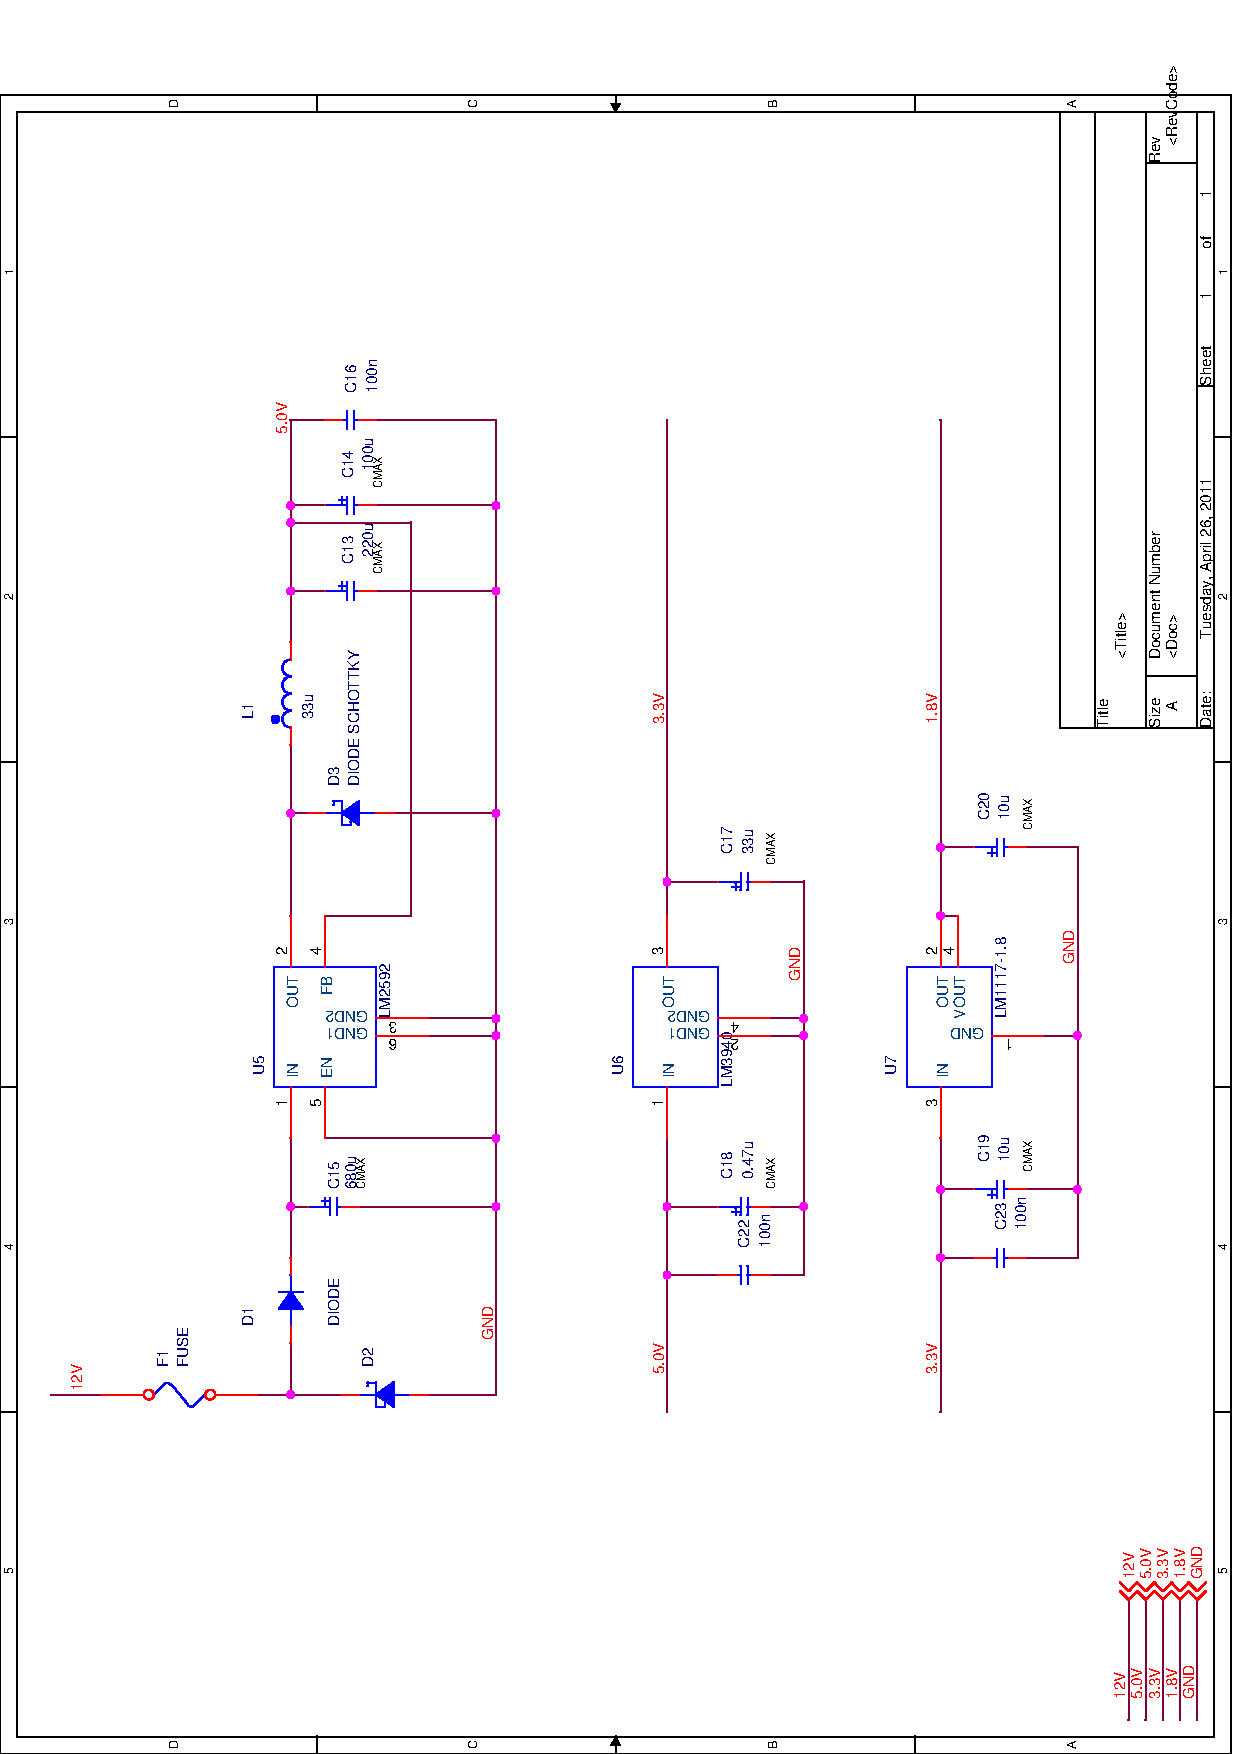
\includegraphics[scale=0.50]{images/final_powersupply.png}
		\caption{Power Supply Section}\label{fig:powersupply_board}
	\end{figure}

	\begin{figure}[H]
		\centering
		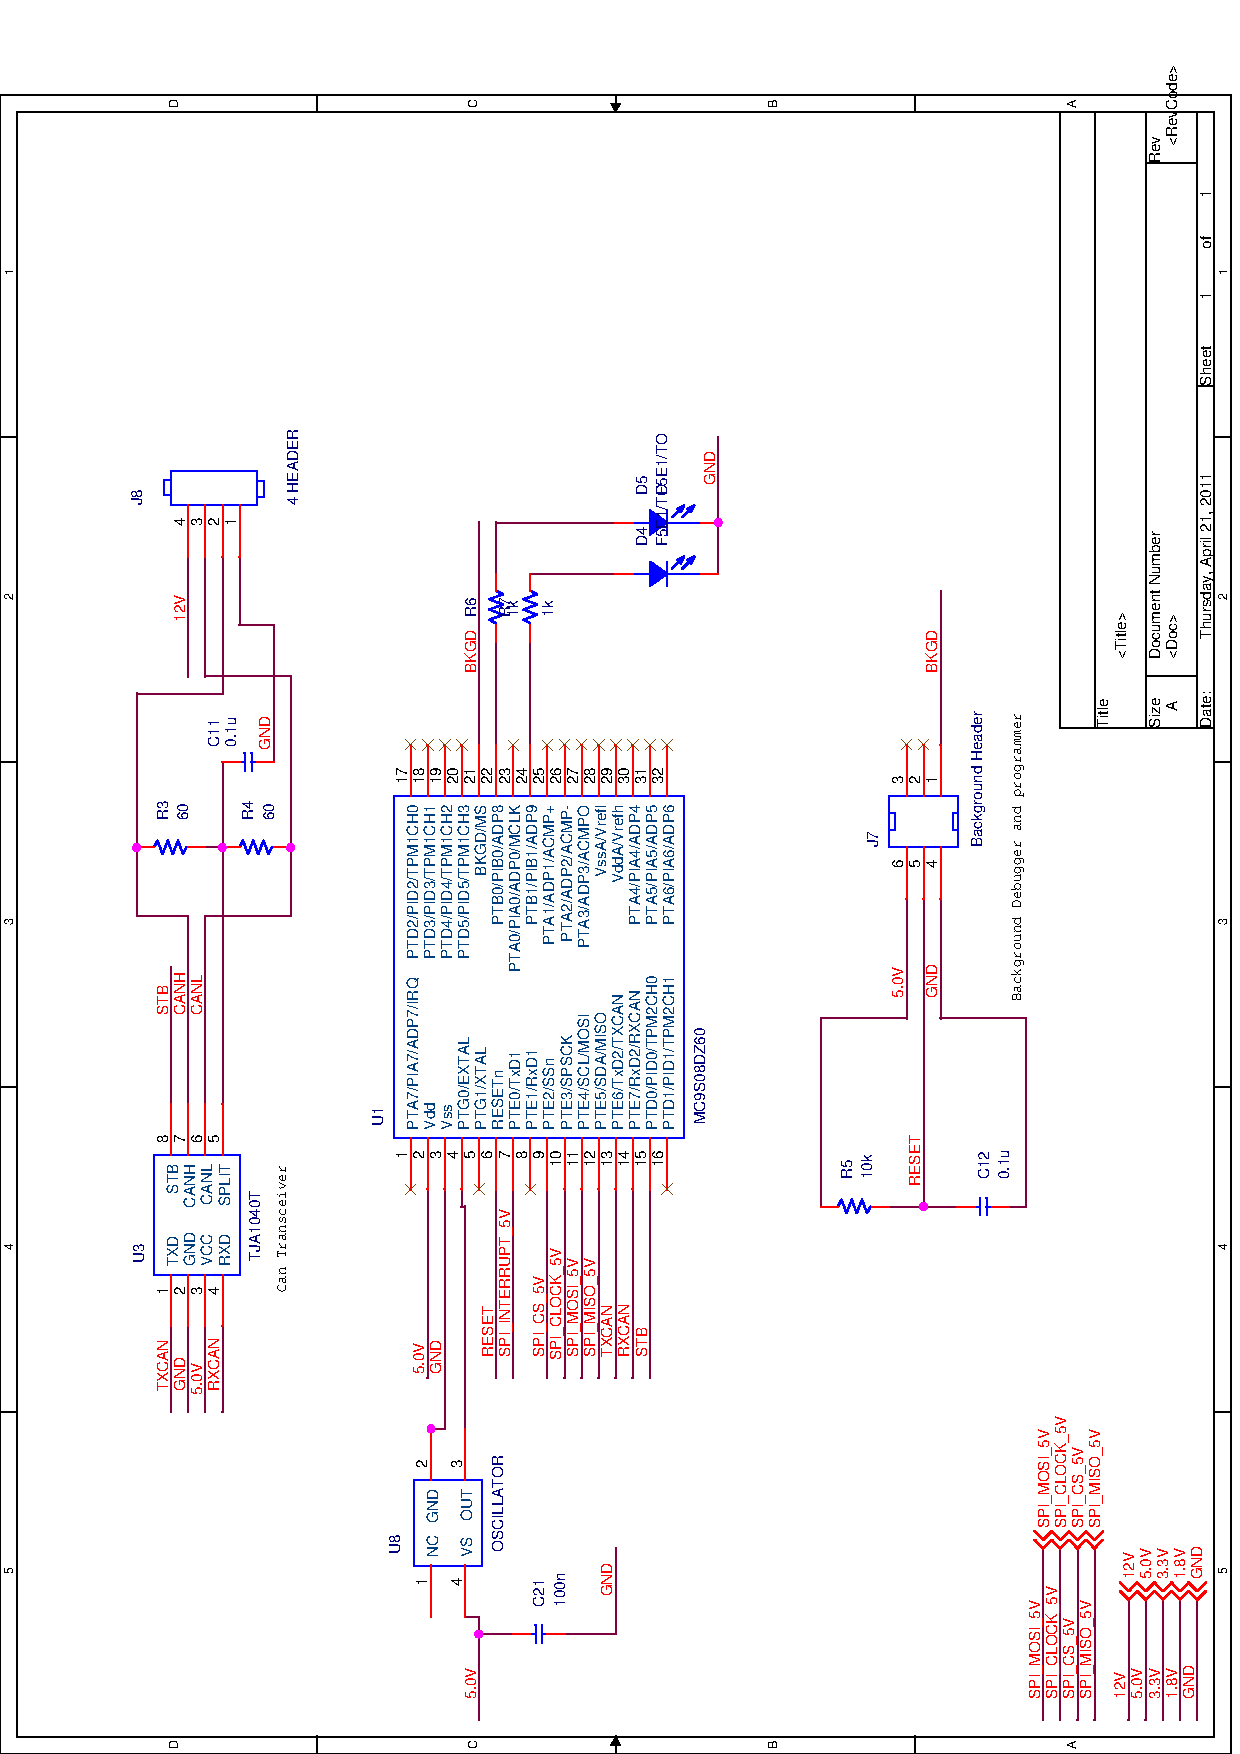
\includegraphics[scale=0.50]{images/final_s08.png}
		\caption{MC9S08 Section}\label{fig:s08_board}
	\end{figure}

	\begin{figure}[H]
		\centering
		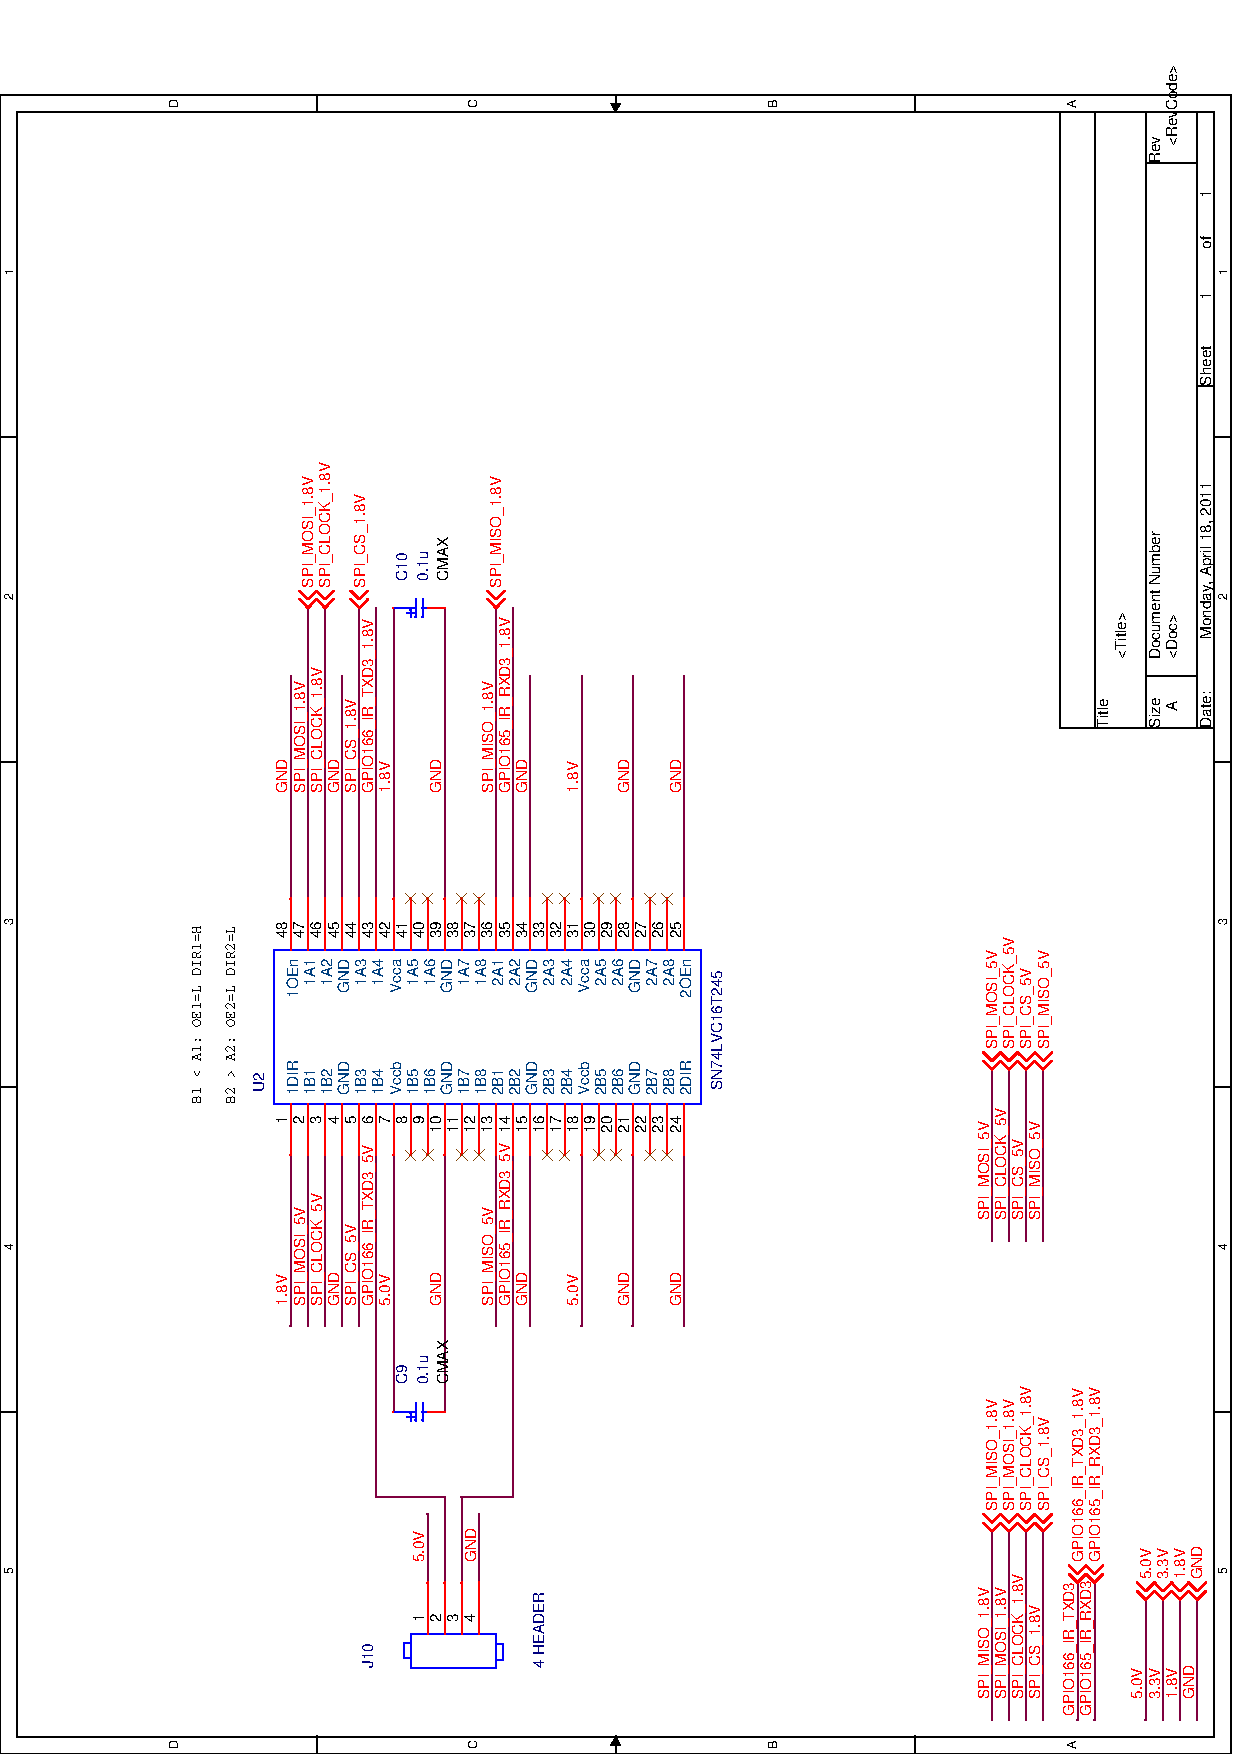
\includegraphics[scale=0.50]{images/final_sn74.png}
		\caption{SN74 Section}\label{fig:finalsn74_board}
	\end{figure}

	\begin{figure}[H]
		\centering
		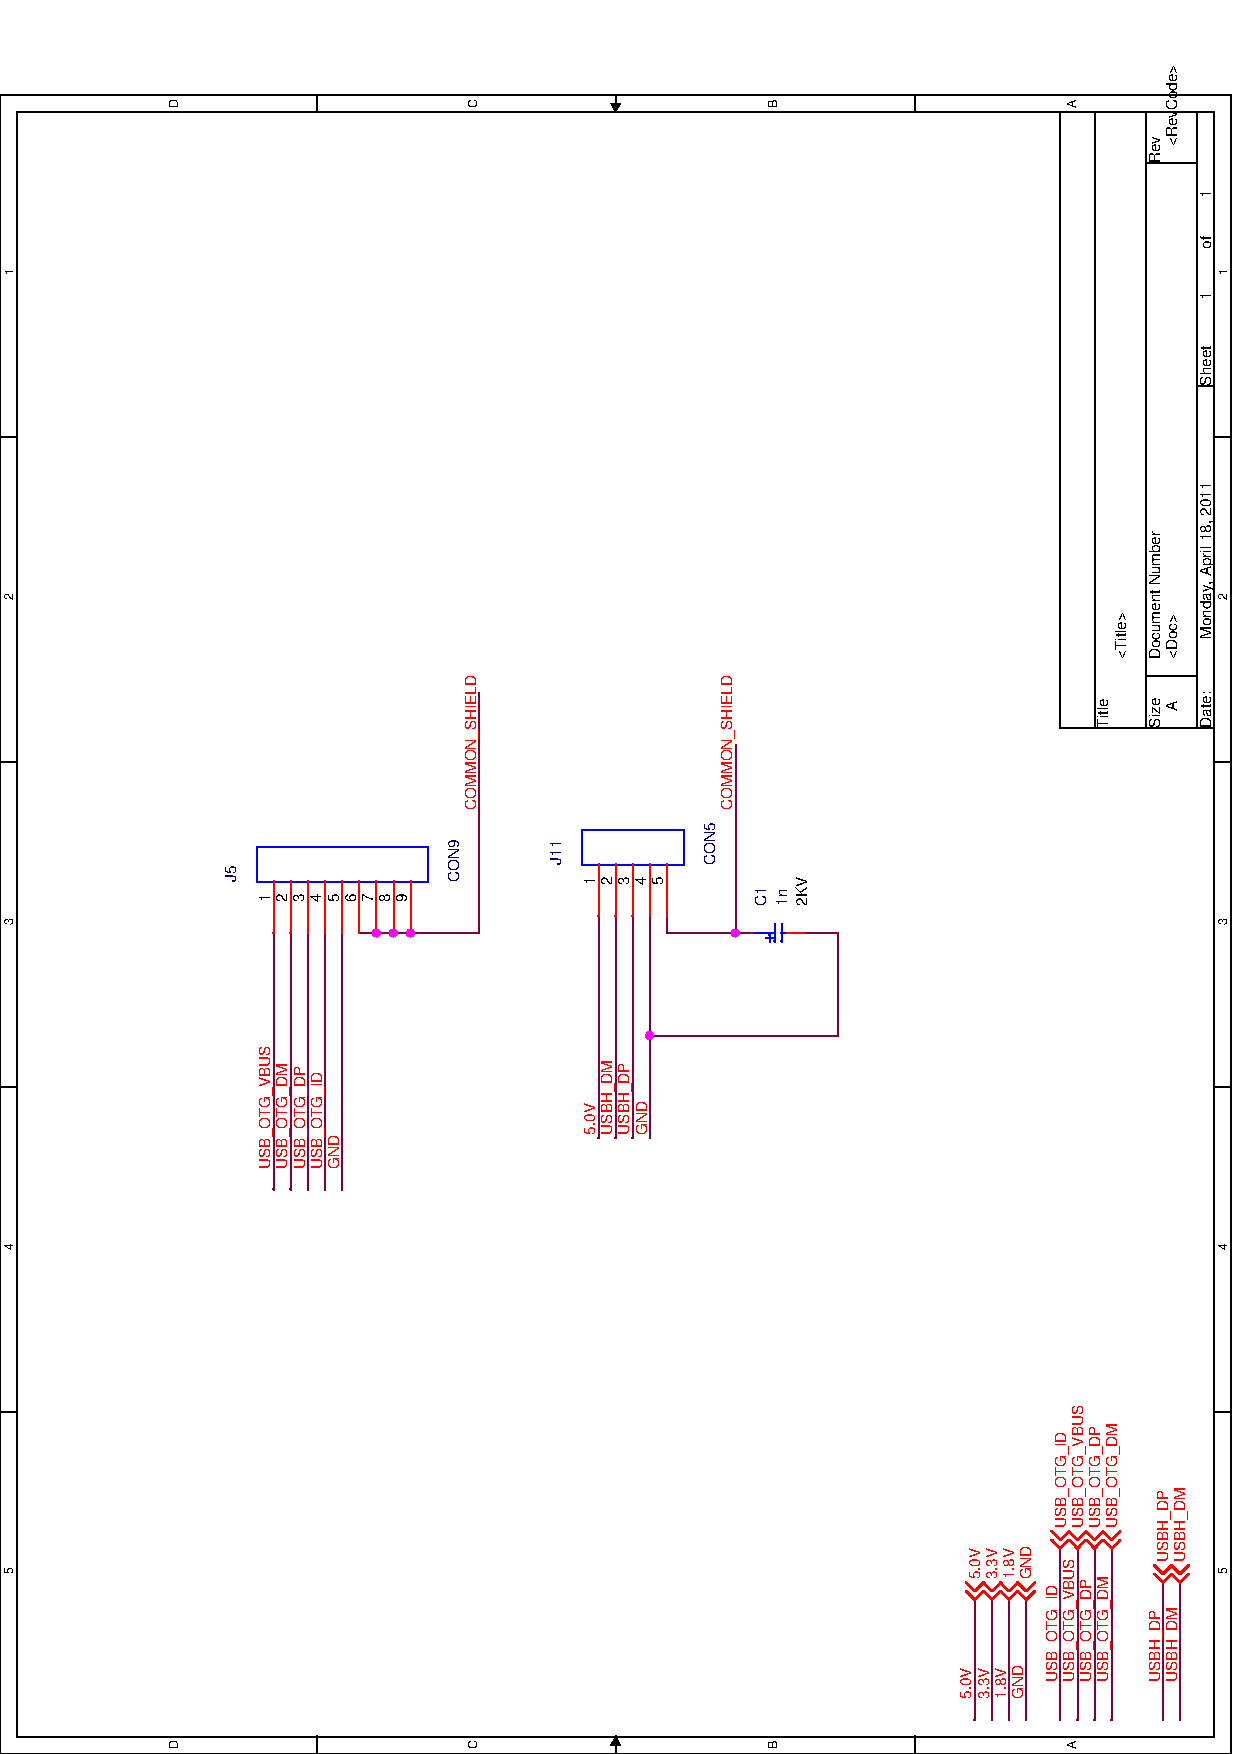
\includegraphics[scale=0.50]{images/final_usb.png}
		\caption{USB Section}\label{fig:usb_board}
	\end{figure}
	
\chapter{LEADSoft Display Manual}

This is the manual for the LEADSoft display program. It entails instructions on how to use the software
and what to expect when the program is running.

\section {Startup}

When the Gumstix receives power it lights up. If the USB screen is properly plugged in
then the back light is switched on. After the screen and its drivers have been intiliased by the Gumstix,
a green light is displayed after which the gumstix proceeds to display booting activity.

\section{Buttons}
Four hardware buttons are used in this project: They are
\begin{itemize}
\item Up
\item Down
\item left/back
\item right/enter
\end{itemize}

\section {Running Program}
The program runs automatically on successfull system bootup. If the system is connected to the CAN network
then the display shows some of the values from the CAN network. Otherwise it stays still.

\subsection{Gear Up/Down}
While the program is in the display mode (i.e displaying the widgets that are updated), the up down arrow keys
can be used to send CAN gear up and CAN gear down packets resepctively to the CAN network. This only happens when 
in the display mode.


\subsection{Menu}
To open the menu window the right/enter button is pressed. The menu window should popup. Menu items can be selected
by using the right/enter key.

The left/back key is used to move to the previous menu window while up and down keys are used to navigate both ways around a menu window.

The GUI has been designed to be fully intuitive and as such should be easy to navigate around and understand.		
	
\subsection {Display}	
	The icons on the buttom right of the screen represent oil temperature and coolant temperature respectively.

\chapter{Cost Breakdown}
	\begin{tabular}{|c|c|c|c|}
	\hline
	Part & Unit Cost & Quantity & Subtotal\\
	\hline
	Gumstix Overo Earth & \$149 & 1 & £91\\
	
	70 pin dock connectors & \$5 & 5 & £15.14\\

	MC9CS08DZ60 & £6.62 & 2 & £13.24\\

	Green LED & £0.07 & 3 & £0.21\\

	Various Resistors & £Varied & 54 & £1.44\\

	Schottky rectifier & £0.08 & 2 & £0.16\\

	USB mini AB & £1.22 & 2 & £2.44\\

	33 $\mu$H Inductor & £2.84 & 1 & £2.84\\

	MAX232 Driver Receiver & £0.71 & 1 & £0.71\\

	TVS Diode & £0.125 & 2 & £0.25\\

	16MHz Crystal Osc & £4.83 & 1 & £4.83\\

	Bulgin W/proof USB & £6.71 & 1 & £6.71\\

	Fast Fuse & £0.555 & 2 & £1.11\\

	USB cap & £0.59 & 1 & £0.59\\

	Various Capacitors & £Varied & 42 & £20.07\\

	SN74 Level Shifter & £0.50 & 3 & £1.50\\

	LM2592MVS 5V & £3.35 & 1 & £3.35\\

	LM3940 3.3V & £1.59 & 1 & £1.59\\
	\hline
	& & TOTAL & £152.04\\
	\hline
	\end{tabular}
	
\chapter{Linux Kernel Configuration}
	\section{Configuring Linux}
	\subsection{Introduction}
		\indent This section will explain how to set up a linux distribution
		from scratch on the gumstix that is compatible with the project board.
		The process of creating a working linux system is tricky
		and requires some knowledges on how to use command line based commands.
		The instructions will explain how to set up {\bf OpenEmbedded} cross
		compilation system, how to configure and compile the linux kernel and
		how to configure the outcoming linux system. The compilation of
		everything from scratch is time consuming and the initial compilation
		of the OpenEmbedded packages took about 24hours on a virtual machine.

	\subsection{OpenEmbedded}
	\subsubsection{What is OpenEmbedded ?}
		Openembedded is a build framework for embedded devices running Linux.
		It offers a suit of tools and packages to allow developers to create a
		complete Linux distribution for the target device. Bitbake ``recipes''
		are included to provide a configuration-less deployment of packages to
		different architectures.

	\subsubsection{Prerequisites}
		\begin{itemize}	
			\item A recent Linux distribution, Linux Mint 10 has been used 
			during the project

			\item Distribution packages: git, subversion, gcc, patch, help2man,
			diffstat, texi2html, makeinfo (texinfo on Linux Mint/Ubuntu),
			ncurses-devel (libncurses5-dev on Linux Mint/Ubuntu), cvs, gawk,
			python-dev, python-pysqlite2, unzip, chrpath, ccache and 
			python-psyco (recommended).
		\end{itemize}

		Note: On some distributions the {\bf /bin/sh} file is a symbolic link
		to  {\bf /bin/dash}, to restore sh to the standard shell run
		{\bf dpkg-reconfigure dash} as super-user and answer {\bf NO} when
		asked whether you want to install dash as {\bf /bin/sh}.

	\subsubsection{Retrieving the source code}
		The Gumstix documentation on OpenEmbedded recommend at least 10GB of
		free space on the hard disk however during the project a dedicated 
		linux install has been used and 50GB of hard disk were required for
		the compilation plus the Linux distribution.\\
		\\
		The default gumstix OpenEmbedded configuration uses the {\bf overo-oe}
		folder in the home folder of the current user this can be modified but
		will not be explain in this document.
		\\
		First create the ``overo-oe'' folder and cd into it.
\begin{lstlisting}
	$ mkdir -p ~/overo-oe
	$ cd ~/overo-oe
\end{lstlisting}
		
		Now to retrieve the Gumstix Overo OpenEmbedded solution, this will take
		some time depending on your internet connection.
\begin{lstlisting}
	$ git clone git://gitorious.org/gumstix-oe/mainline.git\
		org.openembedded.dev

	$ cd org.openembedded.dev
	$ git checkout --track -b overo origin/overo
\end{lstlisting}
		
		Next step is to install BitBake.
\begin{lstlisting}
	$ cd ..
	$ git clone git://git.openembedded.net/bitbake bitbake
	$ cd bitbake
	$ git checkout 1.10.2
\end{lstlisting}
		
	\subsubsection{Environment setup}
		Create the OpenEmbedded configuration files and profile based on the
		provided files.
\begin{lstlisting}
	$ cp -r org.openembedded.dev/contrib/gumstix/build .
\end{lstlisting}
		
		Setup the environment variables on the bash profiles (assuming bash is
		the shell used).
\begin{lstlisting}
	$ cat ~/overo-oe/build/profile >> ~/.bashrc
\end{lstlisting}

	\subsubsection{First Build}	
		You can build a basic kernel and non-gui root file system now, this
		task will take a long time depending on the internet connection as the
		packages required will be downloaded on the fly and also depending on
		the computer speed. Only the first compilation will take so much time
		and the next ones will used the precompiled packages.
		 One issue has been identifier on the University
		network at this stage, wget program is used to download some of the
		source code and does not apply the proxy settings. (a workaround can
		be used but is not in the scope of this document).\\
		\\
		Run the build process
\begin{lstlisting}
	$ cd ~/overo-oe
	$ bitbake omap3-console-image
\end{lstlisting}
		
		Once the compilation is over the root file system and kernel image
		will be located in {\bf ~/overo-oe/tmp/deploy/glibc/images/overo}
	
	\section{Preparing the microSD Card}
	\subsection{Partitioning the card}
		The microSD card have to be formatted in a specific way to allow the
		gumstix to boot on it.
		\\
		Identify the micro sd device
\begin{lstlisting}
	$ fdisk -l
\end{lstlisting}
		Assuming the micro sd device is {\bf /dev/sdb}\\
		Unmount the device
\begin{lstlisting}
	$ umount /dev/sdb
\end{lstlisting}
		Create an empty partition table
\begin{lstlisting}
	$ sudo fdisk /dev/sdb
	Command (m for help): o
	Building a new DOS disklabel. Changes will remain in memory only,
	until you decide to write them. After that, of course, the previous
	content won't be recoverable.
	Warning: invalid flag 0x0000 of partition table 4 will be corrected by w(rite)
\end{lstlisting}
		Look at the current card informations
\begin{lstlisting}
	Command (m for help): p
	Disk /dev/sdb: 2032 MB, 2032664576 bytes
	64 heads, 63 sectors/track, 984 cylinders
	Units = cylinders of 4032 * 512 = 2064384 bytes
	Disk identifier: 0x00aa8e5c
	Device Boot      Start         End      Blocks   Id  System
\end{lstlisting}
		Note the card size in bytes (i.e 2032664576)\\
		Switch to ``Expert'' mode:
\begin{lstlisting}
	Command (m for help): x
\end{lstlisting}
		To allow the gumstix to boot from the sd card the geometry needs to be
		255 heads and 63 sectors with 512 bytes per sector therefore the number
		of cylinders have to be calculated.\\
		\begin{center}
			{\bf card\_number\_of\_bytes / 255 / 63 / 512 = number\_of\_cylinders}
		\end{center}
		This value have to be round {\bf down} and not up. In the case of the
		SD card shown above the number\_of\_cylinders is 247.
\begin{lstlisting}
	Expert command (m for help): h
	Number of heads (1-256, default 4): 255
	Expert command (m for help): s
	Number of sectors (1-63, default 62): 63
	Warning: setting sector offset for DOS compatiblity
	Expert command (m for help): c
	Number of cylinders (1-1048576, default 984): number_of_cylinders
\end{lstlisting}
		Return to fdisk main mode and create the two partitions that will be
		used by the kernel and by the root file system (rootfs).\\

		Create a 32MB FAT partition
\begin{lstlisting}
	Expert command (m for help): r
	Command (m for help): n
	Command action
	e   extended
	p   primary partition (1-4)
	p
	Partition number (1-4): 1
	First cylinder (1-247, default 1): 1
	Last cylinder or +size or +sizeM or +sizeK (1-247, default 15): +32M
\end{lstlisting}

		Change the partition to FAT32
\begin{lstlisting}
	Command (m for help): t
	Selected partition 1
	Hex code (type L to list codes): c
	Changed system type of partition 1 to c (W95 FAT32 (LBA))
\end{lstlisting}

		Make it bootable
\begin{lstlisting}
	Command (m for help): a
	Partition number (1-4): 1
\end{lstlisting}

		Create the ext3 partition for the rootfs
\begin{lstlisting}
	Command (m for help): n
	Command action
	e   extended
	p   primary partition (1-4)
	p
	Partition number (1-4): 2
	First cylinder (6-247, default 6): 6
	Last cylinder or +size or +sizeM or +sizeK (6-247, default 247): 247
\end{lstlisting}

		Verify the new partition info
\begin{lstlisting}
	Command (m for help): p
	Disk /dev/sdb: 2032 MB, 2032664576 bytes
	255 heads, 63 sectors/track, 247 cylinders
	Units = cylinders of 16065 * 512 = 8225280 bytes
	Disk identifier: 0x00aa8e5c
	Device Boot      Start         End      Blocks   Id  System
	/dev/sdb1   *           1           5       40131    c  W95 FAT32 (LBA)
	/dev/sdb2               6         247     1943865   83  Linux
\end{lstlisting}

		Write the new partition table onto the card
\begin{lstlisting}
	Command (m for help): w
	The partition table has been altered!
	Calling ioctl() to re-read partition table.
	WARNING: If you have created or modified any DOS 6.x
	partitions, please see the fdisk manual page for additional
	information.
	Syncing disks
\end{lstlisting}

	\subsection{Formatting the new partitions}
		Create the two paritions file systems
\begin{lstlisting}
	$ sudo mkfs.vfat -F 32 /dev/sdb1 -n FAT
		...
	$ sudo mkfs.ext3 /dev/sdb2
		...
\end{lstlisting}

	\subsection{Installing the system on the SD card}
		There are three files required of the FAT partition to boot the gumstix
		that should have been compiled during the OpenEmbedded compilation
		stage.
		\begin{itemize}
			\item MLO: the boot-loader loader
			\item u-boot.bin: the boot-loader
			\item uImage: the Linux Kernel
		\end{itemize}

		Mount the FAT partition and copy the MLO {\bf first}.
\begin{lstlisting}
	$ sudo mount /dev/sdb1 /media/card
	$ sudo cp MLO-overo /media/card/MLO
	$ sudo cp u-boot.bin /media/card/u-boot.bin
	$ sudo cp uImage /media/card/uImage
\end{lstlisting}

		Unmount the FAT partition and mount the ext3 one
\begin{lstlisting}
	$ sudo umount /dev/sdb1
	$ sudo mount /dev/sdb2 /media/card
\end{lstlisting}

		Untar the rootfs
\begin{lstlisting}
	$ cd /media/card
	$ sudo tar xvaf /path/to/console-image.tar.bz2
\end{lstlisting}

		Unmount the ext3 partition
\begin{lstlisting}
	$ umount /dev/sdb2
\end{lstlisting}

		At this point you should have a bootable linux on the gumstix however
		the screen will not work without configuration but the linux can be
		accessed through the serial communication.

	\section{Compiling a custom kernel on the Gumstix}
		This section assumes that a Linux distribution is already up and
		running on the Gumstix and that a serial communication through the TTY
		connection is established.

		\subsection{Retrieving the kernel source code}
		The easiest way to retrieve the last version with the already applied
		patches for the gumstix is to use there GIT repository to checkout the
		files.\\
		Open the file {\bf linux-omap3\_2.6.36.bb} from the OpenEmbedded files
		and look for SRC\_URI the address next to it. During the project
		development the URI was git://www.sakoman.com/git/linux-omap-2.6.git
		therefore open a Terminal clone the repository.
\begin{lstlisting}
	$ git clone -n git://www.sakoman.com/git/linux-omap-2.6.git linux-omap
	$ cd linux-omap
	$ git branch -a
	 ...
	$ git checkout -b omap-2.6.36 origin/omap-2.6.36
\end{lstlisting}
		Next copy the OpenEmbedded kernel config in the linux kernel source 
		directory.
\begin{lstlisting}
	$ cp ~/overo-oe/org.openembedded.dev/recipes/linux/linux-omap3-2.6.36/defconfig .config
\end{lstlisting}
		Copy this files into a removeable media and connect it to the gumstix.

		\subsection{Configuring the Kernel}
		The Linux kernel have to be configured before it can be compiled
\begin{lstlisting}
	$  make menuconfig
\end{lstlisting}
		This will run the Linux kernel configuration menu, for this board to
		work with the USB screen the displaylink kernel have to be added as
		modules. Other options such as the CAN support have to be enabled.\\
		\\
		To compile the kernel with the DisplayLink drivers for the screen
\begin{lstlisting}
Device Drivers > Staging Drivers > Untick Exclude Staging drivers from being built
Device Drivers > Staging Drivers > Press M on Displaylink USB Framebuffer support
\end{lstlisting}

		To compile the kernel with the CAN support
\begin{lstlisting}
Networking Support > press M on CAN bus subsystem support
Netowrking Support > CAN bus subsystem support > press M on Raw CAN Protocol
Netowrking Support > CAN bus subsystem support > press M on Broadcast Manager CAN Protocol
\end{lstlisting}

		To add the support for the push buttons two files have to be modified,
		the u-boot (linux bootloader) multiplexing file to select the function
		of the microcontroller pins and the board configuration in the kernel.\\

		U-Boot Modifications: On the OpenEmbedded system open
		~/overo-oe/tmp/work/overo-angstrom-linux-gnueabi/u-boot-omap3-(version+git-commit)/git/board/overo/overo.h and change the pin definition. The different options for 
		each pin are defined OMAP35X Technical Reference Manual in Section 7.4.4.3

		Kernel Modifications: Open {\bf arch/arm/mach-omap2/board-overo.c} with
		a text editor and search for the definition of gpio\_buttons[]
		an entry such as the following should be added to the array for a
		button to work. A pin can have only one function at a time so make sure
		that the pin is not already assigned.

\begin{lstlisting}
{
	.code			= KEY_UP,	// Send a KEY_UP event
	.gpio			= 19,		// Use pin 19
	.active_low		= 1,		// The button is active low
	.desc			= "key up",	
	.wakeup			= 1,		// Allow this button to wake from sleep
	.decounce_interval	= 20,		// 20ms Decounce delay
},
\end{lstlisting}

\chapter{Code Listings}

\end{document}
